\documentclass[twoside]{book}

% Packages required by doxygen
\usepackage{fixltx2e}
\usepackage{calc}
\usepackage{doxygen}
\usepackage[export]{adjustbox} % also loads graphicx
\usepackage{graphicx}
\usepackage[utf8]{inputenc}
\usepackage{makeidx}
\usepackage{multicol}
\usepackage{multirow}
\PassOptionsToPackage{warn}{textcomp}
\usepackage{textcomp}
\usepackage[nointegrals]{wasysym}
\usepackage[table]{xcolor}

% Font selection
\usepackage[T1]{fontenc}
\usepackage[scaled=.90]{helvet}
\usepackage{courier}
\usepackage{amssymb}
\usepackage{sectsty}
\renewcommand{\familydefault}{\sfdefault}
\allsectionsfont{%
  \fontseries{bc}\selectfont%
  \color{darkgray}%
}
\renewcommand{\DoxyLabelFont}{%
  \fontseries{bc}\selectfont%
  \color{darkgray}%
}
\newcommand{\+}{\discretionary{\mbox{\scriptsize$\hookleftarrow$}}{}{}}

% Page & text layout
\usepackage{geometry}
\geometry{%
  a4paper,%
  top=2.5cm,%
  bottom=2.5cm,%
  left=2.5cm,%
  right=2.5cm%
}
\tolerance=750
\hfuzz=15pt
\hbadness=750
\setlength{\emergencystretch}{15pt}
\setlength{\parindent}{0cm}
\setlength{\parskip}{3ex plus 2ex minus 2ex}
\makeatletter
\renewcommand{\paragraph}{%
  \@startsection{paragraph}{4}{0ex}{-1.0ex}{1.0ex}{%
    \normalfont\normalsize\bfseries\SS@parafont%
  }%
}
\renewcommand{\subparagraph}{%
  \@startsection{subparagraph}{5}{0ex}{-1.0ex}{1.0ex}{%
    \normalfont\normalsize\bfseries\SS@subparafont%
  }%
}
\makeatother

% Headers & footers
\usepackage{fancyhdr}
\pagestyle{fancyplain}
\fancyhead[LE]{\fancyplain{}{\bfseries\thepage}}
\fancyhead[CE]{\fancyplain{}{}}
\fancyhead[RE]{\fancyplain{}{\bfseries\leftmark}}
\fancyhead[LO]{\fancyplain{}{\bfseries\rightmark}}
\fancyhead[CO]{\fancyplain{}{}}
\fancyhead[RO]{\fancyplain{}{\bfseries\thepage}}
\fancyfoot[LE]{\fancyplain{}{}}
\fancyfoot[CE]{\fancyplain{}{}}
\fancyfoot[RE]{\fancyplain{}{\bfseries\scriptsize Generated by Doxygen }}
\fancyfoot[LO]{\fancyplain{}{\bfseries\scriptsize Generated by Doxygen }}
\fancyfoot[CO]{\fancyplain{}{}}
\fancyfoot[RO]{\fancyplain{}{}}
\renewcommand{\footrulewidth}{0.4pt}
\renewcommand{\chaptermark}[1]{%
  \markboth{#1}{}%
}
\renewcommand{\sectionmark}[1]{%
  \markright{\thesection\ #1}%
}

% Indices & bibliography
\usepackage{natbib}
\usepackage[titles]{tocloft}
\setcounter{tocdepth}{3}
\setcounter{secnumdepth}{5}
\makeindex

% Hyperlinks (required, but should be loaded last)
\usepackage{ifpdf}
\ifpdf
  \usepackage[pdftex,pagebackref=true]{hyperref}
\else
  \usepackage[ps2pdf,pagebackref=true]{hyperref}
\fi
\hypersetup{%
  colorlinks=true,%
  linkcolor=blue,%
  citecolor=blue,%
  unicode%
}

% Custom commands
\newcommand{\clearemptydoublepage}{%
  \newpage{\pagestyle{empty}\cleardoublepage}%
}

\usepackage{caption}
\captionsetup{labelsep=space,justification=centering,font={bf},singlelinecheck=off,skip=4pt,position=top}

%===== C O N T E N T S =====

\begin{document}

% Titlepage & ToC
\hypersetup{pageanchor=false,
             bookmarksnumbered=true,
             pdfencoding=unicode
            }
\pagenumbering{roman}
\begin{titlepage}
\vspace*{7cm}
\begin{center}%
{\Large Assignment 3 of the Experimental Robotics Lab course. \\[1ex]\large 1.\+0 }\\
\vspace*{1cm}
{\large Generated by Doxygen 1.8.11}\\
\end{center}
\end{titlepage}
\clearemptydoublepage
\tableofcontents
\clearemptydoublepage
\pagenumbering{arabic}
\hypersetup{pageanchor=true}

%--- Begin generated contents ---
\chapter{Namespace Index}
\section{Packages}
Here are the packages with brief descriptions (if available)\+:\begin{DoxyCompactList}
\item\contentsline{section}{\hyperlink{namespaceballDetection}{ball\+Detection} }{\pageref{namespaceballDetection}}{}
\item\contentsline{section}{\hyperlink{namespacecmdManager}{cmd\+Manager} }{\pageref{namespacecmdManager}}{}
\item\contentsline{section}{\hyperlink{namespacehumanInterface}{human\+Interface} }{\pageref{namespacehumanInterface}}{}
\item\contentsline{section}{\hyperlink{namespaceknowledgeRep}{knowledge\+Rep} }{\pageref{namespaceknowledgeRep}}{}
\item\contentsline{section}{\hyperlink{namespacetrackingBall}{tracking\+Ball} }{\pageref{namespacetrackingBall}}{}
\end{DoxyCompactList}

\chapter{Hierarchical Index}
\section{Class Hierarchy}
This inheritance list is sorted roughly, but not completely, alphabetically\+:\begin{DoxyCompactList}
\item \contentsline{section}{ball\+Detection.\+ball\+Detector}{\pageref{classballDetection_1_1ballDetector}}{}
\item object\begin{DoxyCompactList}
\item \contentsline{section}{tracking\+Ball.\+Tracking}{\pageref{classtrackingBall_1_1Tracking}}{}
\end{DoxyCompactList}
\item \contentsline{section}{knowledge\+Rep.\+Rooms}{\pageref{classknowledgeRep_1_1Rooms}}{}
\item State\begin{DoxyCompactList}
\item \contentsline{section}{cmd\+Manager.\+Find}{\pageref{classcmdManager_1_1Find}}{}
\item \contentsline{section}{cmd\+Manager.\+Normal}{\pageref{classcmdManager_1_1Normal}}{}
\item \contentsline{section}{cmd\+Manager.\+Play}{\pageref{classcmdManager_1_1Play}}{}
\item \contentsline{section}{cmd\+Manager.\+Sleep}{\pageref{classcmdManager_1_1Sleep}}{}
\item \contentsline{section}{cmd\+Manager.\+Track}{\pageref{classcmdManager_1_1Track}}{}
\end{DoxyCompactList}
\end{DoxyCompactList}

\chapter{Class Index}
\section{Class List}
Here are the classes, structs, unions and interfaces with brief descriptions\+:\begin{DoxyCompactList}
\item\contentsline{section}{\hyperlink{classballDetection_1_1ballDetector}{ball\+Detection.\+ball\+Detector} \\*Class which define the color detection algorithm used which run in a node on his own }{\pageref{classballDetection_1_1ballDetector}}{}
\item\contentsline{section}{\hyperlink{classcmdManager_1_1Find}{cmd\+Manager.\+Find} }{\pageref{classcmdManager_1_1Find}}{}
\item\contentsline{section}{\hyperlink{classcmdManager_1_1Normal}{cmd\+Manager.\+Normal} }{\pageref{classcmdManager_1_1Normal}}{}
\item\contentsline{section}{\hyperlink{classcmdManager_1_1Play}{cmd\+Manager.\+Play} }{\pageref{classcmdManager_1_1Play}}{}
\item\contentsline{section}{\hyperlink{classknowledgeRep_1_1Rooms}{knowledge\+Rep.\+Rooms} \\*Class which contain the knowledg representation, for each room name we have a releated color, position and a boolean which notify if the rooms has been detected or not }{\pageref{classknowledgeRep_1_1Rooms}}{}
\item\contentsline{section}{\hyperlink{classcmdManager_1_1Sleep}{cmd\+Manager.\+Sleep} }{\pageref{classcmdManager_1_1Sleep}}{}
\item\contentsline{section}{\hyperlink{classcmdManager_1_1Track}{cmd\+Manager.\+Track} }{\pageref{classcmdManager_1_1Track}}{}
\item\contentsline{section}{\hyperlink{classtrackingBall_1_1Tracking}{tracking\+Ball.\+Tracking} \\*Class used for tracking the balls detected by ball\+Detect.\+py }{\pageref{classtrackingBall_1_1Tracking}}{}
\end{DoxyCompactList}

\chapter{File Index}
\section{File List}
Here is a list of all files with brief descriptions\+:\begin{DoxyCompactList}
\item\contentsline{section}{/root/\+Desktop/catkin\+\_\+ws/src/exp\+\_\+assignment3/scripts/\hyperlink{ballDetection_8py}{ball\+Detection.\+py} }{\pageref{ballDetection_8py}}{}
\item\contentsline{section}{/root/\+Desktop/catkin\+\_\+ws/src/exp\+\_\+assignment3/scripts/\hyperlink{cmdManager_8py}{cmd\+Manager.\+py} }{\pageref{cmdManager_8py}}{}
\item\contentsline{section}{/root/\+Desktop/catkin\+\_\+ws/src/exp\+\_\+assignment3/scripts/\hyperlink{humanInterface_8py}{human\+Interface.\+py} }{\pageref{humanInterface_8py}}{}
\item\contentsline{section}{/root/\+Desktop/catkin\+\_\+ws/src/exp\+\_\+assignment3/scripts/\hyperlink{knowledgeRep_8py}{knowledge\+Rep.\+py} }{\pageref{knowledgeRep_8py}}{}
\item\contentsline{section}{/root/\+Desktop/catkin\+\_\+ws/src/exp\+\_\+assignment3/scripts/\hyperlink{trackingBall_8py}{tracking\+Ball.\+py} \\*This script is used for tracking the balls after the detection, and is responsable of the movement towards the ball of the robot }{\pageref{trackingBall_8py}}{}
\end{DoxyCompactList}

\chapter{Namespace Documentation}
\hypertarget{namespaceballDetection}{}\section{ball\+Detection Namespace Reference}
\label{namespaceballDetection}\index{ball\+Detection@{ball\+Detection}}
\subsection*{Classes}
\begin{DoxyCompactItemize}
\item 
class \hyperlink{classballDetection_1_1ballDetector}{ball\+Detector}
\begin{DoxyCompactList}\small\item\em Class which define the color detection algorithm used which run in a node on his own. \end{DoxyCompactList}\end{DoxyCompactItemize}
\subsection*{Functions}
\begin{DoxyCompactItemize}
\item 
def \hyperlink{namespaceballDetection_af90d57b7d5fbbaa648ba3ba524d541dd}{detection\+State} (state, rd)
\begin{DoxyCompactList}\small\item\em This is the callback function of the subscriber to  topic, it receive a boolen which notify to start the detection or stop it. \end{DoxyCompactList}\item 
def \hyperlink{namespaceballDetection_a8193b8aef394c20f60fadbaeacdafdc0}{main} (args)
\end{DoxyCompactItemize}
\subsection*{Variables}
\begin{DoxyCompactItemize}
\item 
tuple \hyperlink{namespaceballDetection_a39a98090c55ec606030abf18d6820366}{black\+Lower} = (0, 0, 0)
\item 
tuple \hyperlink{namespaceballDetection_a23ab917df5c9f52915a32ec50221f14f}{black\+Upper} = (5,50,50)
\item 
tuple \hyperlink{namespaceballDetection_a92ef9da6121e329eb1703494c3104863}{red\+Lower} = (0, 50, 50)
\item 
tuple \hyperlink{namespaceballDetection_aa460677a3e1cdb2341aeba5fd17aa2b6}{red\+Upper} = (5, 255, 255)
\item 
tuple \hyperlink{namespaceballDetection_a13f45d6a550517a155e1b28fbb1e21b5}{yellow\+Lower} = (25, 50, 50)
\item 
tuple \hyperlink{namespaceballDetection_aaf6f118d96c2df97f6779017e31994af}{yellow\+Upper} = (35, 255, 255)
\item 
tuple \hyperlink{namespaceballDetection_a9baf8ab116194ae3b105440b2331765c}{green\+Lower} = (50, 50, 50)
\item 
tuple \hyperlink{namespaceballDetection_a1132c3cfcdb75ebb1e6ee6318c4caf2d}{green\+Upper} = (70, 255, 255)
\item 
tuple \hyperlink{namespaceballDetection_a7c95f76d92a79c2eba518529d4585fbe}{blue\+Lower} = (100, 50, 50)
\item 
tuple \hyperlink{namespaceballDetection_a32646e670c980662c55d776abcd8615e}{blue\+Upper} = (130, 255, 255)
\item 
tuple \hyperlink{namespaceballDetection_ac513c92adbc3a5f8325877d042cf28fb}{magenta\+Lower} = (125, 50, 50)
\item 
tuple \hyperlink{namespaceballDetection_a3d5c34f17eec8c6b35c650d34409cf6e}{magenta\+Upper} = (150, 255, 255)
\end{DoxyCompactItemize}


\subsection{Function Documentation}
\index{ball\+Detection@{ball\+Detection}!detection\+State@{detection\+State}}
\index{detection\+State@{detection\+State}!ball\+Detection@{ball\+Detection}}
\subsubsection[{\texorpdfstring{detection\+State(state, rd)}{detectionState(state, rd)}}]{\setlength{\rightskip}{0pt plus 5cm}def ball\+Detection.\+detection\+State (
\begin{DoxyParamCaption}
\item[{}]{state, }
\item[{}]{rd}
\end{DoxyParamCaption}
)}\hypertarget{namespaceballDetection_af90d57b7d5fbbaa648ba3ba524d541dd}{}\label{namespaceballDetection_af90d57b7d5fbbaa648ba3ba524d541dd}


This is the callback function of the subscriber to  topic, it receive a boolen which notify to start the detection or stop it. 

\index{ball\+Detection@{ball\+Detection}!main@{main}}
\index{main@{main}!ball\+Detection@{ball\+Detection}}
\subsubsection[{\texorpdfstring{main(args)}{main(args)}}]{\setlength{\rightskip}{0pt plus 5cm}def ball\+Detection.\+main (
\begin{DoxyParamCaption}
\item[{}]{args}
\end{DoxyParamCaption}
)}\hypertarget{namespaceballDetection_a8193b8aef394c20f60fadbaeacdafdc0}{}\label{namespaceballDetection_a8193b8aef394c20f60fadbaeacdafdc0}


\subsection{Variable Documentation}
\index{ball\+Detection@{ball\+Detection}!black\+Lower@{black\+Lower}}
\index{black\+Lower@{black\+Lower}!ball\+Detection@{ball\+Detection}}
\subsubsection[{\texorpdfstring{black\+Lower}{blackLower}}]{\setlength{\rightskip}{0pt plus 5cm}tuple ball\+Detection.\+black\+Lower = (0, 0, 0)}\hypertarget{namespaceballDetection_a39a98090c55ec606030abf18d6820366}{}\label{namespaceballDetection_a39a98090c55ec606030abf18d6820366}
\index{ball\+Detection@{ball\+Detection}!black\+Upper@{black\+Upper}}
\index{black\+Upper@{black\+Upper}!ball\+Detection@{ball\+Detection}}
\subsubsection[{\texorpdfstring{black\+Upper}{blackUpper}}]{\setlength{\rightskip}{0pt plus 5cm}tuple ball\+Detection.\+black\+Upper = (5,50,50)}\hypertarget{namespaceballDetection_a23ab917df5c9f52915a32ec50221f14f}{}\label{namespaceballDetection_a23ab917df5c9f52915a32ec50221f14f}
\index{ball\+Detection@{ball\+Detection}!blue\+Lower@{blue\+Lower}}
\index{blue\+Lower@{blue\+Lower}!ball\+Detection@{ball\+Detection}}
\subsubsection[{\texorpdfstring{blue\+Lower}{blueLower}}]{\setlength{\rightskip}{0pt plus 5cm}tuple ball\+Detection.\+blue\+Lower = (100, 50, 50)}\hypertarget{namespaceballDetection_a7c95f76d92a79c2eba518529d4585fbe}{}\label{namespaceballDetection_a7c95f76d92a79c2eba518529d4585fbe}
\index{ball\+Detection@{ball\+Detection}!blue\+Upper@{blue\+Upper}}
\index{blue\+Upper@{blue\+Upper}!ball\+Detection@{ball\+Detection}}
\subsubsection[{\texorpdfstring{blue\+Upper}{blueUpper}}]{\setlength{\rightskip}{0pt plus 5cm}tuple ball\+Detection.\+blue\+Upper = (130, 255, 255)}\hypertarget{namespaceballDetection_a32646e670c980662c55d776abcd8615e}{}\label{namespaceballDetection_a32646e670c980662c55d776abcd8615e}
\index{ball\+Detection@{ball\+Detection}!green\+Lower@{green\+Lower}}
\index{green\+Lower@{green\+Lower}!ball\+Detection@{ball\+Detection}}
\subsubsection[{\texorpdfstring{green\+Lower}{greenLower}}]{\setlength{\rightskip}{0pt plus 5cm}tuple ball\+Detection.\+green\+Lower = (50, 50, 50)}\hypertarget{namespaceballDetection_a9baf8ab116194ae3b105440b2331765c}{}\label{namespaceballDetection_a9baf8ab116194ae3b105440b2331765c}
\index{ball\+Detection@{ball\+Detection}!green\+Upper@{green\+Upper}}
\index{green\+Upper@{green\+Upper}!ball\+Detection@{ball\+Detection}}
\subsubsection[{\texorpdfstring{green\+Upper}{greenUpper}}]{\setlength{\rightskip}{0pt plus 5cm}tuple ball\+Detection.\+green\+Upper = (70, 255, 255)}\hypertarget{namespaceballDetection_a1132c3cfcdb75ebb1e6ee6318c4caf2d}{}\label{namespaceballDetection_a1132c3cfcdb75ebb1e6ee6318c4caf2d}
\index{ball\+Detection@{ball\+Detection}!magenta\+Lower@{magenta\+Lower}}
\index{magenta\+Lower@{magenta\+Lower}!ball\+Detection@{ball\+Detection}}
\subsubsection[{\texorpdfstring{magenta\+Lower}{magentaLower}}]{\setlength{\rightskip}{0pt plus 5cm}tuple ball\+Detection.\+magenta\+Lower = (125, 50, 50)}\hypertarget{namespaceballDetection_ac513c92adbc3a5f8325877d042cf28fb}{}\label{namespaceballDetection_ac513c92adbc3a5f8325877d042cf28fb}
\index{ball\+Detection@{ball\+Detection}!magenta\+Upper@{magenta\+Upper}}
\index{magenta\+Upper@{magenta\+Upper}!ball\+Detection@{ball\+Detection}}
\subsubsection[{\texorpdfstring{magenta\+Upper}{magentaUpper}}]{\setlength{\rightskip}{0pt plus 5cm}tuple ball\+Detection.\+magenta\+Upper = (150, 255, 255)}\hypertarget{namespaceballDetection_a3d5c34f17eec8c6b35c650d34409cf6e}{}\label{namespaceballDetection_a3d5c34f17eec8c6b35c650d34409cf6e}
\index{ball\+Detection@{ball\+Detection}!red\+Lower@{red\+Lower}}
\index{red\+Lower@{red\+Lower}!ball\+Detection@{ball\+Detection}}
\subsubsection[{\texorpdfstring{red\+Lower}{redLower}}]{\setlength{\rightskip}{0pt plus 5cm}tuple ball\+Detection.\+red\+Lower = (0, 50, 50)}\hypertarget{namespaceballDetection_a92ef9da6121e329eb1703494c3104863}{}\label{namespaceballDetection_a92ef9da6121e329eb1703494c3104863}
\index{ball\+Detection@{ball\+Detection}!red\+Upper@{red\+Upper}}
\index{red\+Upper@{red\+Upper}!ball\+Detection@{ball\+Detection}}
\subsubsection[{\texorpdfstring{red\+Upper}{redUpper}}]{\setlength{\rightskip}{0pt plus 5cm}tuple ball\+Detection.\+red\+Upper = (5, 255, 255)}\hypertarget{namespaceballDetection_aa460677a3e1cdb2341aeba5fd17aa2b6}{}\label{namespaceballDetection_aa460677a3e1cdb2341aeba5fd17aa2b6}
\index{ball\+Detection@{ball\+Detection}!yellow\+Lower@{yellow\+Lower}}
\index{yellow\+Lower@{yellow\+Lower}!ball\+Detection@{ball\+Detection}}
\subsubsection[{\texorpdfstring{yellow\+Lower}{yellowLower}}]{\setlength{\rightskip}{0pt plus 5cm}tuple ball\+Detection.\+yellow\+Lower = (25, 50, 50)}\hypertarget{namespaceballDetection_a13f45d6a550517a155e1b28fbb1e21b5}{}\label{namespaceballDetection_a13f45d6a550517a155e1b28fbb1e21b5}
\index{ball\+Detection@{ball\+Detection}!yellow\+Upper@{yellow\+Upper}}
\index{yellow\+Upper@{yellow\+Upper}!ball\+Detection@{ball\+Detection}}
\subsubsection[{\texorpdfstring{yellow\+Upper}{yellowUpper}}]{\setlength{\rightskip}{0pt plus 5cm}tuple ball\+Detection.\+yellow\+Upper = (35, 255, 255)}\hypertarget{namespaceballDetection_aaf6f118d96c2df97f6779017e31994af}{}\label{namespaceballDetection_aaf6f118d96c2df97f6779017e31994af}

\hypertarget{namespacecmdManager}{}\section{cmd\+Manager Namespace Reference}
\label{namespacecmdManager}\index{cmd\+Manager@{cmd\+Manager}}
\subsection*{Classes}
\begin{DoxyCompactItemize}
\item 
class \hyperlink{classcmdManager_1_1Find}{Find}
\item 
class \hyperlink{classcmdManager_1_1Normal}{Normal}
\item 
class \hyperlink{classcmdManager_1_1Play}{Play}
\item 
class \hyperlink{classcmdManager_1_1Sleep}{Sleep}
\item 
class \hyperlink{classcmdManager_1_1Track}{Track}
\end{DoxyCompactItemize}
\subsection*{Functions}
\begin{DoxyCompactItemize}
\item 
def \hyperlink{namespacecmdManager_a62a68181d751176538db8063d7b11987}{detection\+\_\+routine} (color)
\begin{DoxyCompactList}\small\item\em Callback of the ball\+\_\+detection\+\_\+subscriber, is called any time a new colored ball is found, precisely a new color is given in input and then the function check if the color was already detected, if not the move\+\_\+base client is stopped for start the tracking. \end{DoxyCompactList}\item 
def \hyperlink{namespacecmdManager_a50ab72ebc575eb7032c50d17a6d592c6}{U\+Icallback} (data)
\begin{DoxyCompactList}\small\item\em Callback of the human interface, each time a user command is received the function change the P\+L\+AY flag and the message is parsed. \end{DoxyCompactList}\item 
def \hyperlink{namespacecmdManager_ac53d2d1248b660039d5a90768ff3bd5e}{go\+\_\+to} (x, y)
\begin{DoxyCompactList}\small\item\em Function which implement the navigation to given input position using the move\+\_\+base action server. \end{DoxyCompactList}\item 
def \hyperlink{namespacecmdManager_a3e64a5e295736776673178e6ff94d1e5}{main} ()
\end{DoxyCompactItemize}
\subsection*{Variables}
\begin{DoxyCompactItemize}
\item 
\hyperlink{namespacecmdManager_ad1967c9cd71b2174a9b4c56d32f08fcc}{client} = actionlib.\+Simple\+Action\+Client(\textquotesingle{}move\+\_\+base\textquotesingle{},Move\+Base\+Action)
\begin{DoxyCompactList}\small\item\em Initialized the client to the move\+\_\+base action server for moving the robot. \end{DoxyCompactList}\item 
\hyperlink{namespacecmdManager_a5f10b08efaeaad88cf34e075895f4d9d}{R\+D\+\_\+pub} = rospy.\+Publisher(\textquotesingle{}detection\+\_\+state\textquotesingle{}, Bool, queue\+\_\+size=10)
\begin{DoxyCompactList}\small\item\em Initialized publisher of the detection state which is a boolean (active or not). \end{DoxyCompactList}\item 
\hyperlink{namespacecmdManager_a783b0ef84682af39dc9f2b8e828c4ad9}{rooms} = \hyperlink{classknowledgeRep_1_1Rooms}{Rooms}()
\begin{DoxyCompactList}\small\item\em Initialized object of the class Rooms() for use the knowledge representation defined in \hyperlink{knowledgeRep_8py}{knowledge\+Rep.\+py}. \end{DoxyCompactList}\item 
dictionary \hyperlink{namespacecmdManager_a927e4211865b745599afe42e9e8d7c8e}{ctrl\+\_\+var} = \{\char`\"{}P\+L\+AY\char`\"{} \+: False, \char`\"{}T\+A\+R\+G\+E\+T\+\_\+\+R\+O\+OM\char`\"{} \+: \char`\"{}None\char`\"{}, \char`\"{}N\+E\+W\+\_\+\+C\+O\+L\+OR\char`\"{} \+: \char`\"{}None\char`\"{}, \char`\"{}F\+I\+ND\char`\"{} \+: False\}
\begin{DoxyCompactList}\small\item\em Dictionary that store important control variables and flags. \end{DoxyCompactList}\end{DoxyCompactItemize}


\subsection{Function Documentation}
\index{cmd\+Manager@{cmd\+Manager}!detection\+\_\+routine@{detection\+\_\+routine}}
\index{detection\+\_\+routine@{detection\+\_\+routine}!cmd\+Manager@{cmd\+Manager}}
\subsubsection[{\texorpdfstring{detection\+\_\+routine(color)}{detection_routine(color)}}]{\setlength{\rightskip}{0pt plus 5cm}def cmd\+Manager.\+detection\+\_\+routine (
\begin{DoxyParamCaption}
\item[{}]{color}
\end{DoxyParamCaption}
)}\hypertarget{namespacecmdManager_a62a68181d751176538db8063d7b11987}{}\label{namespacecmdManager_a62a68181d751176538db8063d7b11987}


Callback of the ball\+\_\+detection\+\_\+subscriber, is called any time a new colored ball is found, precisely a new color is given in input and then the function check if the color was already detected, if not the move\+\_\+base client is stopped for start the tracking. 


\begin{DoxyParams}{Parameters}
{\em color} & is the color detected (string) by the detection algorithm. \\
\hline
\end{DoxyParams}
\index{cmd\+Manager@{cmd\+Manager}!go\+\_\+to@{go\+\_\+to}}
\index{go\+\_\+to@{go\+\_\+to}!cmd\+Manager@{cmd\+Manager}}
\subsubsection[{\texorpdfstring{go\+\_\+to(x, y)}{go_to(x, y)}}]{\setlength{\rightskip}{0pt plus 5cm}def cmd\+Manager.\+go\+\_\+to (
\begin{DoxyParamCaption}
\item[{}]{x, }
\item[{}]{y}
\end{DoxyParamCaption}
)}\hypertarget{namespacecmdManager_ac53d2d1248b660039d5a90768ff3bd5e}{}\label{namespacecmdManager_ac53d2d1248b660039d5a90768ff3bd5e}


Function which implement the navigation to given input position using the move\+\_\+base action server. 


\begin{DoxyParams}{Parameters}
{\em x} & X goal position. \\
\hline
{\em y} & Y goal position. \\
\hline
\end{DoxyParams}
\index{cmd\+Manager@{cmd\+Manager}!main@{main}}
\index{main@{main}!cmd\+Manager@{cmd\+Manager}}
\subsubsection[{\texorpdfstring{main()}{main()}}]{\setlength{\rightskip}{0pt plus 5cm}def cmd\+Manager.\+main (
\begin{DoxyParamCaption}
{}
\end{DoxyParamCaption}
)}\hypertarget{namespacecmdManager_a3e64a5e295736776673178e6ff94d1e5}{}\label{namespacecmdManager_a3e64a5e295736776673178e6ff94d1e5}
\index{cmd\+Manager@{cmd\+Manager}!U\+Icallback@{U\+Icallback}}
\index{U\+Icallback@{U\+Icallback}!cmd\+Manager@{cmd\+Manager}}
\subsubsection[{\texorpdfstring{U\+Icallback(data)}{UIcallback(data)}}]{\setlength{\rightskip}{0pt plus 5cm}def cmd\+Manager.\+U\+Icallback (
\begin{DoxyParamCaption}
\item[{}]{data}
\end{DoxyParamCaption}
)}\hypertarget{namespacecmdManager_a50ab72ebc575eb7032c50d17a6d592c6}{}\label{namespacecmdManager_a50ab72ebc575eb7032c50d17a6d592c6}


Callback of the human interface, each time a user command is received the function change the P\+L\+AY flag and the message is parsed. 


\begin{DoxyParams}{Parameters}
{\em data} & is the message (string). \\
\hline
\end{DoxyParams}


\subsection{Variable Documentation}
\index{cmd\+Manager@{cmd\+Manager}!client@{client}}
\index{client@{client}!cmd\+Manager@{cmd\+Manager}}
\subsubsection[{\texorpdfstring{client}{client}}]{\setlength{\rightskip}{0pt plus 5cm}cmd\+Manager.\+client = actionlib.\+Simple\+Action\+Client(\textquotesingle{}move\+\_\+base\textquotesingle{},Move\+Base\+Action)}\hypertarget{namespacecmdManager_ad1967c9cd71b2174a9b4c56d32f08fcc}{}\label{namespacecmdManager_ad1967c9cd71b2174a9b4c56d32f08fcc}


Initialized the client to the move\+\_\+base action server for moving the robot. 

\index{cmd\+Manager@{cmd\+Manager}!ctrl\+\_\+var@{ctrl\+\_\+var}}
\index{ctrl\+\_\+var@{ctrl\+\_\+var}!cmd\+Manager@{cmd\+Manager}}
\subsubsection[{\texorpdfstring{ctrl\+\_\+var}{ctrl_var}}]{\setlength{\rightskip}{0pt plus 5cm}dictionary cmd\+Manager.\+ctrl\+\_\+var = \{\char`\"{}P\+L\+AY\char`\"{} \+: False, \char`\"{}T\+A\+R\+G\+E\+T\+\_\+\+R\+O\+OM\char`\"{} \+: \char`\"{}None\char`\"{}, \char`\"{}N\+E\+W\+\_\+\+C\+O\+L\+OR\char`\"{} \+: \char`\"{}None\char`\"{}, \char`\"{}F\+I\+ND\char`\"{} \+: False\}}\hypertarget{namespacecmdManager_a927e4211865b745599afe42e9e8d7c8e}{}\label{namespacecmdManager_a927e4211865b745599afe42e9e8d7c8e}


Dictionary that store important control variables and flags. 


\begin{DoxyItemize}
\item P\+L\+AY\+: Flag which notify if there is a P\+L\+AY request
\item T\+A\+R\+G\+E\+T\+\_\+\+R\+O\+OM\+: Control variable which contain the desired room given by the user
\item N\+E\+W\+\_\+\+C\+O\+L\+OR\+: Control variable which contatin a color corresponding to the las detected ball.
\item F\+I\+ND\+: Flag which notify if we are in F\+I\+ND state or not. 
\end{DoxyItemize}\index{cmd\+Manager@{cmd\+Manager}!R\+D\+\_\+pub@{R\+D\+\_\+pub}}
\index{R\+D\+\_\+pub@{R\+D\+\_\+pub}!cmd\+Manager@{cmd\+Manager}}
\subsubsection[{\texorpdfstring{R\+D\+\_\+pub}{RD_pub}}]{\setlength{\rightskip}{0pt plus 5cm}cmd\+Manager.\+R\+D\+\_\+pub = rospy.\+Publisher(\textquotesingle{}detection\+\_\+state\textquotesingle{}, Bool, queue\+\_\+size=10)}\hypertarget{namespacecmdManager_a5f10b08efaeaad88cf34e075895f4d9d}{}\label{namespacecmdManager_a5f10b08efaeaad88cf34e075895f4d9d}


Initialized publisher of the detection state which is a boolean (active or not). 

\index{cmd\+Manager@{cmd\+Manager}!rooms@{rooms}}
\index{rooms@{rooms}!cmd\+Manager@{cmd\+Manager}}
\subsubsection[{\texorpdfstring{rooms}{rooms}}]{\setlength{\rightskip}{0pt plus 5cm}cmd\+Manager.\+rooms = {\bf Rooms}()}\hypertarget{namespacecmdManager_a783b0ef84682af39dc9f2b8e828c4ad9}{}\label{namespacecmdManager_a783b0ef84682af39dc9f2b8e828c4ad9}


Initialized object of the class Rooms() for use the knowledge representation defined in \hyperlink{knowledgeRep_8py}{knowledge\+Rep.\+py}. 


\hypertarget{namespacehumanInterface}{}\section{human\+Interface Namespace Reference}
\label{namespacehumanInterface}\index{human\+Interface@{human\+Interface}}
\subsection*{Functions}
\begin{DoxyCompactItemize}
\item 
def \hyperlink{namespacehumanInterface_a6c8bc8cecea1600244c11ff2f4543075}{human\+Interface} ()
\end{DoxyCompactItemize}
\subsection*{Variables}
\begin{DoxyCompactItemize}
\item 
\hyperlink{namespacehumanInterface_a97ed5bebf33df6316165742f3082bcad}{anonymous}
\end{DoxyCompactItemize}


\subsection{Function Documentation}
\index{human\+Interface@{human\+Interface}!human\+Interface@{human\+Interface}}
\index{human\+Interface@{human\+Interface}!human\+Interface@{human\+Interface}}
\subsubsection[{\texorpdfstring{human\+Interface()}{humanInterface()}}]{\setlength{\rightskip}{0pt plus 5cm}def human\+Interface.\+human\+Interface (
\begin{DoxyParamCaption}
{}
\end{DoxyParamCaption}
)}\hypertarget{namespacehumanInterface_a6c8bc8cecea1600244c11ff2f4543075}{}\label{namespacehumanInterface_a6c8bc8cecea1600244c11ff2f4543075}


\subsection{Variable Documentation}
\index{human\+Interface@{human\+Interface}!anonymous@{anonymous}}
\index{anonymous@{anonymous}!human\+Interface@{human\+Interface}}
\subsubsection[{\texorpdfstring{anonymous}{anonymous}}]{\setlength{\rightskip}{0pt plus 5cm}human\+Interface.\+anonymous}\hypertarget{namespacehumanInterface_a97ed5bebf33df6316165742f3082bcad}{}\label{namespacehumanInterface_a97ed5bebf33df6316165742f3082bcad}

\hypertarget{namespaceknowledgeRep}{}\section{knowledge\+Rep Namespace Reference}
\label{namespaceknowledgeRep}\index{knowledge\+Rep@{knowledge\+Rep}}
\subsection*{Classes}
\begin{DoxyCompactItemize}
\item 
class \hyperlink{classknowledgeRep_1_1Rooms}{Rooms}
\begin{DoxyCompactList}\small\item\em Class which contain the knowledg representation, for each room name we have a releated color, position and a boolean which notify if the rooms has been detected or not. \end{DoxyCompactList}\end{DoxyCompactItemize}

\hypertarget{namespacetrackingBall}{}\section{tracking\+Ball Namespace Reference}
\label{namespacetrackingBall}\index{tracking\+Ball@{tracking\+Ball}}
\subsection*{Classes}
\begin{DoxyCompactItemize}
\item 
class \hyperlink{classtrackingBall_1_1Tracking}{Tracking}
\begin{DoxyCompactList}\small\item\em Class used for tracking the balls detected by ball\+Detect.\+py. \end{DoxyCompactList}\end{DoxyCompactItemize}
\subsection*{Functions}
\begin{DoxyCompactItemize}
\item 
def \hyperlink{namespacetrackingBall_a598e946cfc8046154c148b5a4cc59c85}{main} ()
\end{DoxyCompactItemize}
\subsection*{Variables}
\begin{DoxyCompactItemize}
\item 
tuple \hyperlink{namespacetrackingBall_a01153645a6d9c8883679549bef428084}{black\+Lower} = (0, 0, 0)
\item 
tuple \hyperlink{namespacetrackingBall_aa7ba379d6623121d8177f1fc3ef5034d}{black\+Upper} = (5,50,50)
\item 
tuple \hyperlink{namespacetrackingBall_ac067a86c452c58c5f13931c2ac2561bb}{red\+Lower} = (0, 50, 50)
\item 
tuple \hyperlink{namespacetrackingBall_a20b2aa393ebb9c87978d17185adaf892}{red\+Upper} = (5, 255, 255)
\item 
tuple \hyperlink{namespacetrackingBall_a995cb139bea83c20c743922a0bec5af2}{yellow\+Lower} = (25, 50, 50)
\item 
tuple \hyperlink{namespacetrackingBall_aadefd833712f76b3627f3d4c39f7ba47}{yellow\+Upper} = (35, 255, 255)
\item 
tuple \hyperlink{namespacetrackingBall_aeb72dbd40498c11743fafc005f92f3e7}{green\+Lower} = (50, 50, 50)
\item 
tuple \hyperlink{namespacetrackingBall_ade0b7e73d07db09c50b72324c6ed4d9a}{green\+Upper} = (70, 255, 255)
\item 
tuple \hyperlink{namespacetrackingBall_a1cc45fb4974562c2699e1ef0b1ee2038}{blue\+Lower} = (100, 50, 50)
\item 
tuple \hyperlink{namespacetrackingBall_a92b4c05c5050867894310e92c4ae3d66}{blue\+Upper} = (130, 255, 255)
\item 
tuple \hyperlink{namespacetrackingBall_ae34afbda2818a5105a51c3f883315b6e}{magenta\+Lower} = (125, 50, 50)
\item 
tuple \hyperlink{namespacetrackingBall_aa7fc4609467db9724ea81aa2d6442a41}{magenta\+Upper} = (150, 255, 255)
\end{DoxyCompactItemize}


\subsection{Function Documentation}
\index{tracking\+Ball@{tracking\+Ball}!main@{main}}
\index{main@{main}!tracking\+Ball@{tracking\+Ball}}
\subsubsection[{\texorpdfstring{main()}{main()}}]{\setlength{\rightskip}{0pt plus 5cm}def tracking\+Ball.\+main (
\begin{DoxyParamCaption}
{}
\end{DoxyParamCaption}
)}\hypertarget{namespacetrackingBall_a598e946cfc8046154c148b5a4cc59c85}{}\label{namespacetrackingBall_a598e946cfc8046154c148b5a4cc59c85}


\subsection{Variable Documentation}
\index{tracking\+Ball@{tracking\+Ball}!black\+Lower@{black\+Lower}}
\index{black\+Lower@{black\+Lower}!tracking\+Ball@{tracking\+Ball}}
\subsubsection[{\texorpdfstring{black\+Lower}{blackLower}}]{\setlength{\rightskip}{0pt plus 5cm}tuple tracking\+Ball.\+black\+Lower = (0, 0, 0)}\hypertarget{namespacetrackingBall_a01153645a6d9c8883679549bef428084}{}\label{namespacetrackingBall_a01153645a6d9c8883679549bef428084}
\index{tracking\+Ball@{tracking\+Ball}!black\+Upper@{black\+Upper}}
\index{black\+Upper@{black\+Upper}!tracking\+Ball@{tracking\+Ball}}
\subsubsection[{\texorpdfstring{black\+Upper}{blackUpper}}]{\setlength{\rightskip}{0pt plus 5cm}tuple tracking\+Ball.\+black\+Upper = (5,50,50)}\hypertarget{namespacetrackingBall_aa7ba379d6623121d8177f1fc3ef5034d}{}\label{namespacetrackingBall_aa7ba379d6623121d8177f1fc3ef5034d}
\index{tracking\+Ball@{tracking\+Ball}!blue\+Lower@{blue\+Lower}}
\index{blue\+Lower@{blue\+Lower}!tracking\+Ball@{tracking\+Ball}}
\subsubsection[{\texorpdfstring{blue\+Lower}{blueLower}}]{\setlength{\rightskip}{0pt plus 5cm}tuple tracking\+Ball.\+blue\+Lower = (100, 50, 50)}\hypertarget{namespacetrackingBall_a1cc45fb4974562c2699e1ef0b1ee2038}{}\label{namespacetrackingBall_a1cc45fb4974562c2699e1ef0b1ee2038}
\index{tracking\+Ball@{tracking\+Ball}!blue\+Upper@{blue\+Upper}}
\index{blue\+Upper@{blue\+Upper}!tracking\+Ball@{tracking\+Ball}}
\subsubsection[{\texorpdfstring{blue\+Upper}{blueUpper}}]{\setlength{\rightskip}{0pt plus 5cm}tuple tracking\+Ball.\+blue\+Upper = (130, 255, 255)}\hypertarget{namespacetrackingBall_a92b4c05c5050867894310e92c4ae3d66}{}\label{namespacetrackingBall_a92b4c05c5050867894310e92c4ae3d66}
\index{tracking\+Ball@{tracking\+Ball}!green\+Lower@{green\+Lower}}
\index{green\+Lower@{green\+Lower}!tracking\+Ball@{tracking\+Ball}}
\subsubsection[{\texorpdfstring{green\+Lower}{greenLower}}]{\setlength{\rightskip}{0pt plus 5cm}tuple tracking\+Ball.\+green\+Lower = (50, 50, 50)}\hypertarget{namespacetrackingBall_aeb72dbd40498c11743fafc005f92f3e7}{}\label{namespacetrackingBall_aeb72dbd40498c11743fafc005f92f3e7}
\index{tracking\+Ball@{tracking\+Ball}!green\+Upper@{green\+Upper}}
\index{green\+Upper@{green\+Upper}!tracking\+Ball@{tracking\+Ball}}
\subsubsection[{\texorpdfstring{green\+Upper}{greenUpper}}]{\setlength{\rightskip}{0pt plus 5cm}tuple tracking\+Ball.\+green\+Upper = (70, 255, 255)}\hypertarget{namespacetrackingBall_ade0b7e73d07db09c50b72324c6ed4d9a}{}\label{namespacetrackingBall_ade0b7e73d07db09c50b72324c6ed4d9a}
\index{tracking\+Ball@{tracking\+Ball}!magenta\+Lower@{magenta\+Lower}}
\index{magenta\+Lower@{magenta\+Lower}!tracking\+Ball@{tracking\+Ball}}
\subsubsection[{\texorpdfstring{magenta\+Lower}{magentaLower}}]{\setlength{\rightskip}{0pt plus 5cm}tuple tracking\+Ball.\+magenta\+Lower = (125, 50, 50)}\hypertarget{namespacetrackingBall_ae34afbda2818a5105a51c3f883315b6e}{}\label{namespacetrackingBall_ae34afbda2818a5105a51c3f883315b6e}
\index{tracking\+Ball@{tracking\+Ball}!magenta\+Upper@{magenta\+Upper}}
\index{magenta\+Upper@{magenta\+Upper}!tracking\+Ball@{tracking\+Ball}}
\subsubsection[{\texorpdfstring{magenta\+Upper}{magentaUpper}}]{\setlength{\rightskip}{0pt plus 5cm}tuple tracking\+Ball.\+magenta\+Upper = (150, 255, 255)}\hypertarget{namespacetrackingBall_aa7fc4609467db9724ea81aa2d6442a41}{}\label{namespacetrackingBall_aa7fc4609467db9724ea81aa2d6442a41}
\index{tracking\+Ball@{tracking\+Ball}!red\+Lower@{red\+Lower}}
\index{red\+Lower@{red\+Lower}!tracking\+Ball@{tracking\+Ball}}
\subsubsection[{\texorpdfstring{red\+Lower}{redLower}}]{\setlength{\rightskip}{0pt plus 5cm}tuple tracking\+Ball.\+red\+Lower = (0, 50, 50)}\hypertarget{namespacetrackingBall_ac067a86c452c58c5f13931c2ac2561bb}{}\label{namespacetrackingBall_ac067a86c452c58c5f13931c2ac2561bb}
\index{tracking\+Ball@{tracking\+Ball}!red\+Upper@{red\+Upper}}
\index{red\+Upper@{red\+Upper}!tracking\+Ball@{tracking\+Ball}}
\subsubsection[{\texorpdfstring{red\+Upper}{redUpper}}]{\setlength{\rightskip}{0pt plus 5cm}tuple tracking\+Ball.\+red\+Upper = (5, 255, 255)}\hypertarget{namespacetrackingBall_a20b2aa393ebb9c87978d17185adaf892}{}\label{namespacetrackingBall_a20b2aa393ebb9c87978d17185adaf892}
\index{tracking\+Ball@{tracking\+Ball}!yellow\+Lower@{yellow\+Lower}}
\index{yellow\+Lower@{yellow\+Lower}!tracking\+Ball@{tracking\+Ball}}
\subsubsection[{\texorpdfstring{yellow\+Lower}{yellowLower}}]{\setlength{\rightskip}{0pt plus 5cm}tuple tracking\+Ball.\+yellow\+Lower = (25, 50, 50)}\hypertarget{namespacetrackingBall_a995cb139bea83c20c743922a0bec5af2}{}\label{namespacetrackingBall_a995cb139bea83c20c743922a0bec5af2}
\index{tracking\+Ball@{tracking\+Ball}!yellow\+Upper@{yellow\+Upper}}
\index{yellow\+Upper@{yellow\+Upper}!tracking\+Ball@{tracking\+Ball}}
\subsubsection[{\texorpdfstring{yellow\+Upper}{yellowUpper}}]{\setlength{\rightskip}{0pt plus 5cm}tuple tracking\+Ball.\+yellow\+Upper = (35, 255, 255)}\hypertarget{namespacetrackingBall_aadefd833712f76b3627f3d4c39f7ba47}{}\label{namespacetrackingBall_aadefd833712f76b3627f3d4c39f7ba47}

\chapter{Class Documentation}
\hypertarget{classballDetection_1_1ballDetector}{}\section{ball\+Detection.\+ball\+Detector Class Reference}
\label{classballDetection_1_1ballDetector}\index{ball\+Detection.\+ball\+Detector@{ball\+Detection.\+ball\+Detector}}


Class which define the color detection algorithm used which run in a node on his own.  


\subsection*{Public Member Functions}
\begin{DoxyCompactItemize}
\item 
def \hyperlink{classballDetection_1_1ballDetector_ac87f218abdb03da0143f113695dca5d5}{\+\_\+\+\_\+init\+\_\+\+\_\+} (self)
\item 
def \hyperlink{classballDetection_1_1ballDetector_ada73fa6d070ed2c2be489e7c89c1b6c0}{color\+\_\+detection} (self, hsv\+\_\+min, hsv\+\_\+max, image\+\_\+np)
\begin{DoxyCompactList}\small\item\em Simple color detection, this function return true when a contour of the given input color is founded in the input image. \end{DoxyCompactList}\item 
def \hyperlink{classballDetection_1_1ballDetector_a62a5e77b3c5af1b96c70b2e5037ce4c6}{ball\+\_\+detection} (self, ros\+\_\+image)
\begin{DoxyCompactList}\small\item\em This function implement the ball detection algorithm, given an input image different mask are applied for detect the color of our knowledge representation. \end{DoxyCompactList}\item 
def \hyperlink{classballDetection_1_1ballDetector_a852941442c83f3160bb2cac307f495dc}{start\+Detection} (self)
\begin{DoxyCompactList}\small\item\em Function that start the detection subscribing to the camera topic. \end{DoxyCompactList}\item 
def \hyperlink{classballDetection_1_1ballDetector_ab146dd9d22b2b5eea5103e56181e51c4}{stop\+Detection} (self)
\begin{DoxyCompactList}\small\item\em Function that stop the detection unregistering the camera topic. \end{DoxyCompactList}\end{DoxyCompactItemize}
\subsection*{Public Attributes}
\begin{DoxyCompactItemize}
\item 
\hyperlink{classballDetection_1_1ballDetector_ae7c6db80d37aa2d3f22b0ea9331823d2}{detected\+Balls}
\begin{DoxyCompactList}\small\item\em List for store already detected colors. \end{DoxyCompactList}\item 
\hyperlink{classballDetection_1_1ballDetector_ab09c82e74e052ab38cbfb5ae32c281ac}{ball\+\_\+detection\+\_\+pub}
\begin{DoxyCompactList}\small\item\em The publisher send strings for transfer the new color founded (associated to a room). \end{DoxyCompactList}\item 
\hyperlink{classballDetection_1_1ballDetector_a2078441c3a3cc044e914c90656a9a5e0}{rate}
\item 
\hyperlink{classballDetection_1_1ballDetector_a7e34212f61e96cbdfabe9db9b7c95e16}{ball\+Detected}
\item 
\hyperlink{classballDetection_1_1ballDetector_a80579e1cc221f9c74eafb6cf5a24e132}{camera\+\_\+sub}
\end{DoxyCompactItemize}


\subsection{Detailed Description}
Class which define the color detection algorithm used which run in a node on his own. 

Receive in input compressed images from the camera and then apply a mask of different colors to detect if at least one colored ball is in the scene. It\textquotesingle{}s important to highlight that colors can be detected only once, so after the first detection of the black ball the algorithm is not able to detect other black balls. 

\subsection{Constructor \& Destructor Documentation}
\index{ball\+Detection\+::ball\+Detector@{ball\+Detection\+::ball\+Detector}!\+\_\+\+\_\+init\+\_\+\+\_\+@{\+\_\+\+\_\+init\+\_\+\+\_\+}}
\index{\+\_\+\+\_\+init\+\_\+\+\_\+@{\+\_\+\+\_\+init\+\_\+\+\_\+}!ball\+Detection\+::ball\+Detector@{ball\+Detection\+::ball\+Detector}}
\subsubsection[{\texorpdfstring{\+\_\+\+\_\+init\+\_\+\+\_\+(self)}{__init__(self)}}]{\setlength{\rightskip}{0pt plus 5cm}def ball\+Detection.\+ball\+Detector.\+\_\+\+\_\+init\+\_\+\+\_\+ (
\begin{DoxyParamCaption}
\item[{}]{self}
\end{DoxyParamCaption}
)}\hypertarget{classballDetection_1_1ballDetector_ac87f218abdb03da0143f113695dca5d5}{}\label{classballDetection_1_1ballDetector_ac87f218abdb03da0143f113695dca5d5}
\begin{DoxyVerb}INITIALIZE ROS NODE and PUBLISHER \end{DoxyVerb}
 

\subsection{Member Function Documentation}
\index{ball\+Detection\+::ball\+Detector@{ball\+Detection\+::ball\+Detector}!ball\+\_\+detection@{ball\+\_\+detection}}
\index{ball\+\_\+detection@{ball\+\_\+detection}!ball\+Detection\+::ball\+Detector@{ball\+Detection\+::ball\+Detector}}
\subsubsection[{\texorpdfstring{ball\+\_\+detection(self, ros\+\_\+image)}{ball_detection(self, ros_image)}}]{\setlength{\rightskip}{0pt plus 5cm}def ball\+Detection.\+ball\+Detector.\+ball\+\_\+detection (
\begin{DoxyParamCaption}
\item[{}]{self, }
\item[{}]{ros\+\_\+image}
\end{DoxyParamCaption}
)}\hypertarget{classballDetection_1_1ballDetector_a62a5e77b3c5af1b96c70b2e5037ce4c6}{}\label{classballDetection_1_1ballDetector_a62a5e77b3c5af1b96c70b2e5037ce4c6}


This function implement the ball detection algorithm, given an input image different mask are applied for detect the color of our knowledge representation. 

It\textquotesingle{}s the callback of the subscriber to the camera topic, so each time a new image is available is called. 
\begin{DoxyParams}{Parameters}
{\em image\+\_\+np} & is the decompressed image and converted in Open\+Cv \\
\hline
\end{DoxyParams}
\index{ball\+Detection\+::ball\+Detector@{ball\+Detection\+::ball\+Detector}!color\+\_\+detection@{color\+\_\+detection}}
\index{color\+\_\+detection@{color\+\_\+detection}!ball\+Detection\+::ball\+Detector@{ball\+Detection\+::ball\+Detector}}
\subsubsection[{\texorpdfstring{color\+\_\+detection(self, hsv\+\_\+min, hsv\+\_\+max, image\+\_\+np)}{color_detection(self, hsv_min, hsv_max, image_np)}}]{\setlength{\rightskip}{0pt plus 5cm}def ball\+Detection.\+ball\+Detector.\+color\+\_\+detection (
\begin{DoxyParamCaption}
\item[{}]{self, }
\item[{}]{hsv\+\_\+min, }
\item[{}]{hsv\+\_\+max, }
\item[{}]{image\+\_\+np}
\end{DoxyParamCaption}
)}\hypertarget{classballDetection_1_1ballDetector_ada73fa6d070ed2c2be489e7c89c1b6c0}{}\label{classballDetection_1_1ballDetector_ada73fa6d070ed2c2be489e7c89c1b6c0}


Simple color detection, this function return true when a contour of the given input color is founded in the input image. 


\begin{DoxyParams}{Parameters}
{\em hsv\+\_\+min} & minimum threshold of the input color expressed in hsv scale. \\
\hline
{\em hsv\+\_\+max} & maximum threshold of the input color expressed in hsv scale. \\
\hline
{\em image\+\_\+np} & image stored in a numpy array. \\
\hline
\end{DoxyParams}
\index{ball\+Detection\+::ball\+Detector@{ball\+Detection\+::ball\+Detector}!start\+Detection@{start\+Detection}}
\index{start\+Detection@{start\+Detection}!ball\+Detection\+::ball\+Detector@{ball\+Detection\+::ball\+Detector}}
\subsubsection[{\texorpdfstring{start\+Detection(self)}{startDetection(self)}}]{\setlength{\rightskip}{0pt plus 5cm}def ball\+Detection.\+ball\+Detector.\+start\+Detection (
\begin{DoxyParamCaption}
\item[{}]{self}
\end{DoxyParamCaption}
)}\hypertarget{classballDetection_1_1ballDetector_a852941442c83f3160bb2cac307f495dc}{}\label{classballDetection_1_1ballDetector_a852941442c83f3160bb2cac307f495dc}


Function that start the detection subscribing to the camera topic. 

\index{ball\+Detection\+::ball\+Detector@{ball\+Detection\+::ball\+Detector}!stop\+Detection@{stop\+Detection}}
\index{stop\+Detection@{stop\+Detection}!ball\+Detection\+::ball\+Detector@{ball\+Detection\+::ball\+Detector}}
\subsubsection[{\texorpdfstring{stop\+Detection(self)}{stopDetection(self)}}]{\setlength{\rightskip}{0pt plus 5cm}def ball\+Detection.\+ball\+Detector.\+stop\+Detection (
\begin{DoxyParamCaption}
\item[{}]{self}
\end{DoxyParamCaption}
)}\hypertarget{classballDetection_1_1ballDetector_ab146dd9d22b2b5eea5103e56181e51c4}{}\label{classballDetection_1_1ballDetector_ab146dd9d22b2b5eea5103e56181e51c4}


Function that stop the detection unregistering the camera topic. 



\subsection{Member Data Documentation}
\index{ball\+Detection\+::ball\+Detector@{ball\+Detection\+::ball\+Detector}!ball\+\_\+detection\+\_\+pub@{ball\+\_\+detection\+\_\+pub}}
\index{ball\+\_\+detection\+\_\+pub@{ball\+\_\+detection\+\_\+pub}!ball\+Detection\+::ball\+Detector@{ball\+Detection\+::ball\+Detector}}
\subsubsection[{\texorpdfstring{ball\+\_\+detection\+\_\+pub}{ball_detection_pub}}]{\setlength{\rightskip}{0pt plus 5cm}ball\+Detection.\+ball\+Detector.\+ball\+\_\+detection\+\_\+pub}\hypertarget{classballDetection_1_1ballDetector_ab09c82e74e052ab38cbfb5ae32c281ac}{}\label{classballDetection_1_1ballDetector_ab09c82e74e052ab38cbfb5ae32c281ac}


The publisher send strings for transfer the new color founded (associated to a room). 

\index{ball\+Detection\+::ball\+Detector@{ball\+Detection\+::ball\+Detector}!ball\+Detected@{ball\+Detected}}
\index{ball\+Detected@{ball\+Detected}!ball\+Detection\+::ball\+Detector@{ball\+Detection\+::ball\+Detector}}
\subsubsection[{\texorpdfstring{ball\+Detected}{ballDetected}}]{\setlength{\rightskip}{0pt plus 5cm}ball\+Detection.\+ball\+Detector.\+ball\+Detected}\hypertarget{classballDetection_1_1ballDetector_a7e34212f61e96cbdfabe9db9b7c95e16}{}\label{classballDetection_1_1ballDetector_a7e34212f61e96cbdfabe9db9b7c95e16}

\begin{DoxyParams}{Parameters}
{\em image\+\_\+np} & is the decompressed image and converted in Open\+Cv \\
\hline
\end{DoxyParams}
\index{ball\+Detection\+::ball\+Detector@{ball\+Detection\+::ball\+Detector}!camera\+\_\+sub@{camera\+\_\+sub}}
\index{camera\+\_\+sub@{camera\+\_\+sub}!ball\+Detection\+::ball\+Detector@{ball\+Detection\+::ball\+Detector}}
\subsubsection[{\texorpdfstring{camera\+\_\+sub}{camera_sub}}]{\setlength{\rightskip}{0pt plus 5cm}ball\+Detection.\+ball\+Detector.\+camera\+\_\+sub}\hypertarget{classballDetection_1_1ballDetector_a80579e1cc221f9c74eafb6cf5a24e132}{}\label{classballDetection_1_1ballDetector_a80579e1cc221f9c74eafb6cf5a24e132}
\index{ball\+Detection\+::ball\+Detector@{ball\+Detection\+::ball\+Detector}!detected\+Balls@{detected\+Balls}}
\index{detected\+Balls@{detected\+Balls}!ball\+Detection\+::ball\+Detector@{ball\+Detection\+::ball\+Detector}}
\subsubsection[{\texorpdfstring{detected\+Balls}{detectedBalls}}]{\setlength{\rightskip}{0pt plus 5cm}ball\+Detection.\+ball\+Detector.\+detected\+Balls}\hypertarget{classballDetection_1_1ballDetector_ae7c6db80d37aa2d3f22b0ea9331823d2}{}\label{classballDetection_1_1ballDetector_ae7c6db80d37aa2d3f22b0ea9331823d2}


List for store already detected colors. 

\index{ball\+Detection\+::ball\+Detector@{ball\+Detection\+::ball\+Detector}!rate@{rate}}
\index{rate@{rate}!ball\+Detection\+::ball\+Detector@{ball\+Detection\+::ball\+Detector}}
\subsubsection[{\texorpdfstring{rate}{rate}}]{\setlength{\rightskip}{0pt plus 5cm}ball\+Detection.\+ball\+Detector.\+rate}\hypertarget{classballDetection_1_1ballDetector_a2078441c3a3cc044e914c90656a9a5e0}{}\label{classballDetection_1_1ballDetector_a2078441c3a3cc044e914c90656a9a5e0}


The documentation for this class was generated from the following file\+:\begin{DoxyCompactItemize}
\item 
/root/\+Desktop/catkin\+\_\+ws/src/exp\+\_\+assignment3/scripts/\hyperlink{ballDetection_8py}{ball\+Detection.\+py}\end{DoxyCompactItemize}

\hypertarget{classcmdManager_1_1Find}{}\section{cmd\+Manager.\+Find Class Reference}
\label{classcmdManager_1_1Find}\index{cmd\+Manager.\+Find@{cmd\+Manager.\+Find}}


Inheritance diagram for cmd\+Manager.\+Find\+:\nopagebreak
\begin{figure}[H]
\begin{center}
\leavevmode
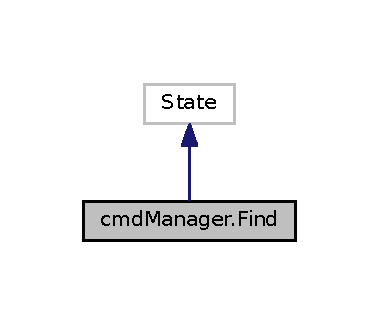
\includegraphics[width=182pt]{classcmdManager_1_1Find__inherit__graph}
\end{center}
\end{figure}


Collaboration diagram for cmd\+Manager.\+Find\+:\nopagebreak
\begin{figure}[H]
\begin{center}
\leavevmode
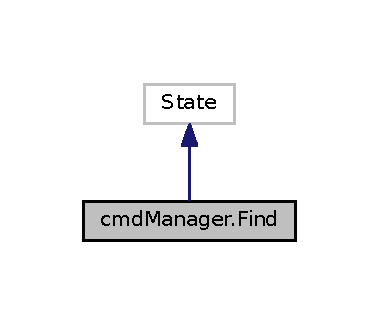
\includegraphics[width=182pt]{classcmdManager_1_1Find__coll__graph}
\end{center}
\end{figure}
\subsection*{Public Member Functions}
\begin{DoxyCompactItemize}
\item 
def \hyperlink{classcmdManager_1_1Find_ac1b5934dd9654da40ee17c6b6680f7b3}{\+\_\+\+\_\+init\+\_\+\+\_\+} (self)
\item 
def \hyperlink{classcmdManager_1_1Find_abd9e8b1f15ff00ebf80384840ec4591b}{execute} (self, userdata)
\end{DoxyCompactItemize}
\subsection*{Public Attributes}
\begin{DoxyCompactItemize}
\item 
\hyperlink{classcmdManager_1_1Find_a35c8ab6f2845c3167b4d9504825b90dd}{rate}
\item 
\hyperlink{classcmdManager_1_1Find_a3e5d82d79af531e17dcc6b68439320ad}{counter}
\end{DoxyCompactItemize}


\subsection{Detailed Description}
\begin{DoxyVerb}Class which define the FIND State of the FSM. In this state the robot explore the area for the requested unknown location during PLAY state.
If a new ball is found then switch to TRACK state, if the ball correspond to the requested room in PLAY state is notified to the user, otherwise 
the new room detected is added in the knowledge. After a while return to PLAY state\end{DoxyVerb}
 

\subsection{Constructor \& Destructor Documentation}
\index{cmd\+Manager\+::\+Find@{cmd\+Manager\+::\+Find}!\+\_\+\+\_\+init\+\_\+\+\_\+@{\+\_\+\+\_\+init\+\_\+\+\_\+}}
\index{\+\_\+\+\_\+init\+\_\+\+\_\+@{\+\_\+\+\_\+init\+\_\+\+\_\+}!cmd\+Manager\+::\+Find@{cmd\+Manager\+::\+Find}}
\subsubsection[{\texorpdfstring{\+\_\+\+\_\+init\+\_\+\+\_\+(self)}{__init__(self)}}]{\setlength{\rightskip}{0pt plus 5cm}def cmd\+Manager.\+Find.\+\_\+\+\_\+init\+\_\+\+\_\+ (
\begin{DoxyParamCaption}
\item[{}]{self}
\end{DoxyParamCaption}
)}\hypertarget{classcmdManager_1_1Find_ac1b5934dd9654da40ee17c6b6680f7b3}{}\label{classcmdManager_1_1Find_ac1b5934dd9654da40ee17c6b6680f7b3}


\subsection{Member Function Documentation}
\index{cmd\+Manager\+::\+Find@{cmd\+Manager\+::\+Find}!execute@{execute}}
\index{execute@{execute}!cmd\+Manager\+::\+Find@{cmd\+Manager\+::\+Find}}
\subsubsection[{\texorpdfstring{execute(self, userdata)}{execute(self, userdata)}}]{\setlength{\rightskip}{0pt plus 5cm}def cmd\+Manager.\+Find.\+execute (
\begin{DoxyParamCaption}
\item[{}]{self, }
\item[{}]{userdata}
\end{DoxyParamCaption}
)}\hypertarget{classcmdManager_1_1Find_abd9e8b1f15ff00ebf80384840ec4591b}{}\label{classcmdManager_1_1Find_abd9e8b1f15ff00ebf80384840ec4591b}


\subsection{Member Data Documentation}
\index{cmd\+Manager\+::\+Find@{cmd\+Manager\+::\+Find}!counter@{counter}}
\index{counter@{counter}!cmd\+Manager\+::\+Find@{cmd\+Manager\+::\+Find}}
\subsubsection[{\texorpdfstring{counter}{counter}}]{\setlength{\rightskip}{0pt plus 5cm}cmd\+Manager.\+Find.\+counter}\hypertarget{classcmdManager_1_1Find_a3e5d82d79af531e17dcc6b68439320ad}{}\label{classcmdManager_1_1Find_a3e5d82d79af531e17dcc6b68439320ad}
\index{cmd\+Manager\+::\+Find@{cmd\+Manager\+::\+Find}!rate@{rate}}
\index{rate@{rate}!cmd\+Manager\+::\+Find@{cmd\+Manager\+::\+Find}}
\subsubsection[{\texorpdfstring{rate}{rate}}]{\setlength{\rightskip}{0pt plus 5cm}cmd\+Manager.\+Find.\+rate}\hypertarget{classcmdManager_1_1Find_a35c8ab6f2845c3167b4d9504825b90dd}{}\label{classcmdManager_1_1Find_a35c8ab6f2845c3167b4d9504825b90dd}


The documentation for this class was generated from the following file\+:\begin{DoxyCompactItemize}
\item 
/root/\+Desktop/catkin\+\_\+ws/src/exp\+\_\+assignment3/scripts/\hyperlink{cmdManager_8py}{cmd\+Manager.\+py}\end{DoxyCompactItemize}

\hypertarget{classcmdManager_1_1Normal}{}\section{cmd\+Manager.\+Normal Class Reference}
\label{classcmdManager_1_1Normal}\index{cmd\+Manager.\+Normal@{cmd\+Manager.\+Normal}}


Inheritance diagram for cmd\+Manager.\+Normal\+:\nopagebreak
\begin{figure}[H]
\begin{center}
\leavevmode
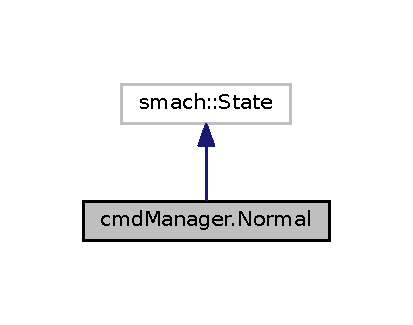
\includegraphics[width=198pt]{classcmdManager_1_1Normal__inherit__graph}
\end{center}
\end{figure}


Collaboration diagram for cmd\+Manager.\+Normal\+:\nopagebreak
\begin{figure}[H]
\begin{center}
\leavevmode
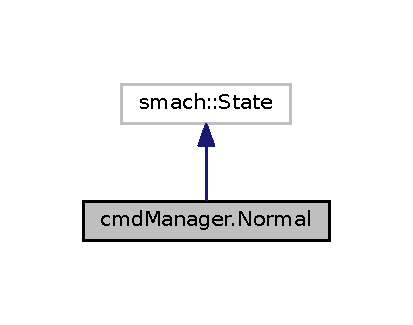
\includegraphics[width=198pt]{classcmdManager_1_1Normal__coll__graph}
\end{center}
\end{figure}
\subsection*{Public Member Functions}
\begin{DoxyCompactItemize}
\item 
def \hyperlink{classcmdManager_1_1Normal_ab492c9d6b86cabc1673e7d128d554c17}{\+\_\+\+\_\+init\+\_\+\+\_\+} (self)
\item 
def \hyperlink{classcmdManager_1_1Normal_a3290ae1ca5346a38bd735b24ed20d359}{execute} (self, userdata)
\end{DoxyCompactItemize}
\subsection*{Public Attributes}
\begin{DoxyCompactItemize}
\item 
\hyperlink{classcmdManager_1_1Normal_ade28669287e8fccab0b4c5cffcc81d35}{rate}
\item 
\hyperlink{classcmdManager_1_1Normal_a83ff274729c38598e1a51d9ffa2871d8}{counter}
\begin{DoxyCompactList}\small\item\em Counter variable to check the number of iteration of the N\+O\+R\+M\+AL state in order to move to S\+L\+E\+EP state after a certain number. \end{DoxyCompactList}\end{DoxyCompactItemize}


\subsection{Detailed Description}
\begin{DoxyVerb}This class defines the NORMAL state of the FSM. In this state random positions are sended to the robot while the PLAY flag
is monitored since if we receive a PLAY command from the user we have to switch state. Moreover it's checked each iteration if 
a new color is detected for switching to TRACK state and also after a predefined number of iteration switch to SLEEP state\end{DoxyVerb}
 

\subsection{Constructor \& Destructor Documentation}
\index{cmd\+Manager\+::\+Normal@{cmd\+Manager\+::\+Normal}!\+\_\+\+\_\+init\+\_\+\+\_\+@{\+\_\+\+\_\+init\+\_\+\+\_\+}}
\index{\+\_\+\+\_\+init\+\_\+\+\_\+@{\+\_\+\+\_\+init\+\_\+\+\_\+}!cmd\+Manager\+::\+Normal@{cmd\+Manager\+::\+Normal}}
\subsubsection[{\texorpdfstring{\+\_\+\+\_\+init\+\_\+\+\_\+(self)}{__init__(self)}}]{\setlength{\rightskip}{0pt plus 5cm}def cmd\+Manager.\+Normal.\+\_\+\+\_\+init\+\_\+\+\_\+ (
\begin{DoxyParamCaption}
\item[{}]{self}
\end{DoxyParamCaption}
)}\hypertarget{classcmdManager_1_1Normal_ab492c9d6b86cabc1673e7d128d554c17}{}\label{classcmdManager_1_1Normal_ab492c9d6b86cabc1673e7d128d554c17}


\subsection{Member Function Documentation}
\index{cmd\+Manager\+::\+Normal@{cmd\+Manager\+::\+Normal}!execute@{execute}}
\index{execute@{execute}!cmd\+Manager\+::\+Normal@{cmd\+Manager\+::\+Normal}}
\subsubsection[{\texorpdfstring{execute(self, userdata)}{execute(self, userdata)}}]{\setlength{\rightskip}{0pt plus 5cm}def cmd\+Manager.\+Normal.\+execute (
\begin{DoxyParamCaption}
\item[{}]{self, }
\item[{}]{userdata}
\end{DoxyParamCaption}
)}\hypertarget{classcmdManager_1_1Normal_a3290ae1ca5346a38bd735b24ed20d359}{}\label{classcmdManager_1_1Normal_a3290ae1ca5346a38bd735b24ed20d359}


\subsection{Member Data Documentation}
\index{cmd\+Manager\+::\+Normal@{cmd\+Manager\+::\+Normal}!counter@{counter}}
\index{counter@{counter}!cmd\+Manager\+::\+Normal@{cmd\+Manager\+::\+Normal}}
\subsubsection[{\texorpdfstring{counter}{counter}}]{\setlength{\rightskip}{0pt plus 5cm}cmd\+Manager.\+Normal.\+counter}\hypertarget{classcmdManager_1_1Normal_a83ff274729c38598e1a51d9ffa2871d8}{}\label{classcmdManager_1_1Normal_a83ff274729c38598e1a51d9ffa2871d8}


Counter variable to check the number of iteration of the N\+O\+R\+M\+AL state in order to move to S\+L\+E\+EP state after a certain number. 

\index{cmd\+Manager\+::\+Normal@{cmd\+Manager\+::\+Normal}!rate@{rate}}
\index{rate@{rate}!cmd\+Manager\+::\+Normal@{cmd\+Manager\+::\+Normal}}
\subsubsection[{\texorpdfstring{rate}{rate}}]{\setlength{\rightskip}{0pt plus 5cm}cmd\+Manager.\+Normal.\+rate}\hypertarget{classcmdManager_1_1Normal_ade28669287e8fccab0b4c5cffcc81d35}{}\label{classcmdManager_1_1Normal_ade28669287e8fccab0b4c5cffcc81d35}


The documentation for this class was generated from the following file\+:\begin{DoxyCompactItemize}
\item 
/root/\+Desktop/catkin\+\_\+ws/src/exp\+\_\+assignment3/scripts/\hyperlink{cmdManager_8py}{cmd\+Manager.\+py}\end{DoxyCompactItemize}

\hypertarget{classcmdManager_1_1Play}{}\section{cmd\+Manager.\+Play Class Reference}
\label{classcmdManager_1_1Play}\index{cmd\+Manager.\+Play@{cmd\+Manager.\+Play}}


Inheritance diagram for cmd\+Manager.\+Play\+:
\nopagebreak
\begin{figure}[H]
\begin{center}
\leavevmode
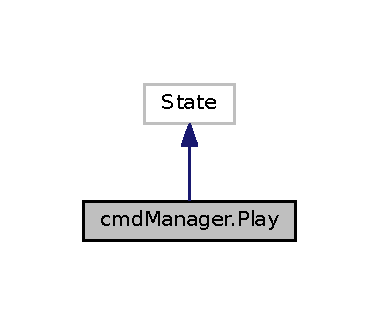
\includegraphics[width=182pt]{classcmdManager_1_1Play__inherit__graph}
\end{center}
\end{figure}


Collaboration diagram for cmd\+Manager.\+Play\+:
\nopagebreak
\begin{figure}[H]
\begin{center}
\leavevmode
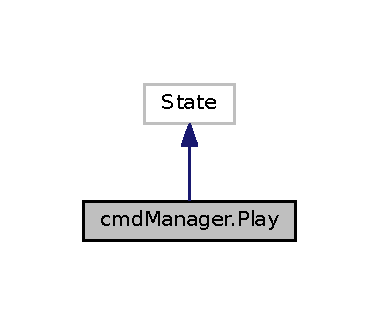
\includegraphics[width=182pt]{classcmdManager_1_1Play__coll__graph}
\end{center}
\end{figure}
\subsection*{Public Member Functions}
\begin{DoxyCompactItemize}
\item 
def \hyperlink{classcmdManager_1_1Play_a4d2579c5fbfe43cfbeb085a149813ed3}{\+\_\+\+\_\+init\+\_\+\+\_\+} (self)
\item 
def \hyperlink{classcmdManager_1_1Play_a6e2839da28e556dc522779a43952eb1a}{execute} (self, userdata)
\end{DoxyCompactItemize}
\subsection*{Public Attributes}
\begin{DoxyCompactItemize}
\item 
\hyperlink{classcmdManager_1_1Play_a8f8e8115f9c44ed73179f6318ab1263a}{rate}
\item 
\hyperlink{classcmdManager_1_1Play_a71ca6215a36ed4a20ed74142d604addb}{counter}
\end{DoxyCompactItemize}


\subsection{Detailed Description}
\begin{DoxyVerb}Class that defines the PLAY state of the FSM. After receiving a PLAY we entered in this state where the robot first goes to the user,
the wait for a target room to reach. If the target room was already discoverd the position associated in the knowledege representation
is reachd, else the robot switch to FIND state. After a while (we count the iterations inside this state) the robot return to NORMAL state.\end{DoxyVerb}
 

\subsection{Constructor \& Destructor Documentation}
\index{cmd\+Manager\+::\+Play@{cmd\+Manager\+::\+Play}!\+\_\+\+\_\+init\+\_\+\+\_\+@{\+\_\+\+\_\+init\+\_\+\+\_\+}}
\index{\+\_\+\+\_\+init\+\_\+\+\_\+@{\+\_\+\+\_\+init\+\_\+\+\_\+}!cmd\+Manager\+::\+Play@{cmd\+Manager\+::\+Play}}
\subsubsection[{\texorpdfstring{\+\_\+\+\_\+init\+\_\+\+\_\+(self)}{__init__(self)}}]{\setlength{\rightskip}{0pt plus 5cm}def cmd\+Manager.\+Play.\+\_\+\+\_\+init\+\_\+\+\_\+ (
\begin{DoxyParamCaption}
\item[{}]{self}
\end{DoxyParamCaption}
)}\hypertarget{classcmdManager_1_1Play_a4d2579c5fbfe43cfbeb085a149813ed3}{}\label{classcmdManager_1_1Play_a4d2579c5fbfe43cfbeb085a149813ed3}


\subsection{Member Function Documentation}
\index{cmd\+Manager\+::\+Play@{cmd\+Manager\+::\+Play}!execute@{execute}}
\index{execute@{execute}!cmd\+Manager\+::\+Play@{cmd\+Manager\+::\+Play}}
\subsubsection[{\texorpdfstring{execute(self, userdata)}{execute(self, userdata)}}]{\setlength{\rightskip}{0pt plus 5cm}def cmd\+Manager.\+Play.\+execute (
\begin{DoxyParamCaption}
\item[{}]{self, }
\item[{}]{userdata}
\end{DoxyParamCaption}
)}\hypertarget{classcmdManager_1_1Play_a6e2839da28e556dc522779a43952eb1a}{}\label{classcmdManager_1_1Play_a6e2839da28e556dc522779a43952eb1a}


\subsection{Member Data Documentation}
\index{cmd\+Manager\+::\+Play@{cmd\+Manager\+::\+Play}!counter@{counter}}
\index{counter@{counter}!cmd\+Manager\+::\+Play@{cmd\+Manager\+::\+Play}}
\subsubsection[{\texorpdfstring{counter}{counter}}]{\setlength{\rightskip}{0pt plus 5cm}cmd\+Manager.\+Play.\+counter}\hypertarget{classcmdManager_1_1Play_a71ca6215a36ed4a20ed74142d604addb}{}\label{classcmdManager_1_1Play_a71ca6215a36ed4a20ed74142d604addb}
\index{cmd\+Manager\+::\+Play@{cmd\+Manager\+::\+Play}!rate@{rate}}
\index{rate@{rate}!cmd\+Manager\+::\+Play@{cmd\+Manager\+::\+Play}}
\subsubsection[{\texorpdfstring{rate}{rate}}]{\setlength{\rightskip}{0pt plus 5cm}cmd\+Manager.\+Play.\+rate}\hypertarget{classcmdManager_1_1Play_a8f8e8115f9c44ed73179f6318ab1263a}{}\label{classcmdManager_1_1Play_a8f8e8115f9c44ed73179f6318ab1263a}


The documentation for this class was generated from the following file\+:\begin{DoxyCompactItemize}
\item 
/root/\+Desktop/catkin\+\_\+ws/src/exp\+\_\+assignment3/scripts/\hyperlink{cmdManager_8py}{cmd\+Manager.\+py}\end{DoxyCompactItemize}

\hypertarget{classknowledgeRep_1_1Rooms}{}\section{knowledge\+Rep.\+Rooms Class Reference}
\label{classknowledgeRep_1_1Rooms}\index{knowledge\+Rep.\+Rooms@{knowledge\+Rep.\+Rooms}}


Class which contain the knowledg representation, for each room name we have a releated color, position and a boolean which notify if the rooms has been detected or not.  


\subsection*{Public Member Functions}
\begin{DoxyCompactItemize}
\item 
def \hyperlink{classknowledgeRep_1_1Rooms_a8b37414da9d2cc9ee820ec306c0b03bf}{\+\_\+\+\_\+init\+\_\+\+\_\+} (self)
\item 
def \hyperlink{classknowledgeRep_1_1Rooms_a834289a5ae57e48cf90087e7f68faba2}{room\+\_\+check} (self, color)
\begin{DoxyCompactList}\small\item\em Function that check if the input color (associated to a particular rooms) was already detected. \end{DoxyCompactList}\item 
def \hyperlink{classknowledgeRep_1_1Rooms_a072ab03a9621d2abd8067817a0583547}{room\+\_\+position} (self, target\+\_\+room)
\begin{DoxyCompactList}\small\item\em Function that returns the position of the given input room. \end{DoxyCompactList}\item 
def \hyperlink{classknowledgeRep_1_1Rooms_a4bdc60738dc11ec176223fe4fb046b2f}{new\+\_\+room} (self, color, x, y)
\begin{DoxyCompactList}\small\item\em Function that check and inform the user if a new room is detected, now the room has a position and the robot know it. \end{DoxyCompactList}\item 
def \hyperlink{classknowledgeRep_1_1Rooms_aaa1ca874182c72929cdd69f5d801ca2e}{room\+\_\+name} (self, x, y)
\begin{DoxyCompactList}\small\item\em Function that return the room name given an input position. \end{DoxyCompactList}\item 
def \hyperlink{classknowledgeRep_1_1Rooms_a41f6960d862a174fce8200ea1c7e003f}{room\+\_\+color} (self, name)
\begin{DoxyCompactList}\small\item\em Function that return the room color given of an input room name. \end{DoxyCompactList}\item 
def \hyperlink{classknowledgeRep_1_1Rooms_ae666c5c43dcaa315e41d7e8de7ae88a2}{random\+\_\+pos} (self)
\begin{DoxyCompactList}\small\item\em Function that generate random positions (inside our house) \end{DoxyCompactList}\item 
def \hyperlink{classknowledgeRep_1_1Rooms_a68eb5ab6fe7ee4edb42c499c14a915c0}{room\+\_\+range} (self, a, l)
\begin{DoxyCompactList}\small\item\em This function receive as input a coordinate and a scalar \char`\"{}l\char`\"{}, returns an array of \char`\"{}l-\/neighborhood\char`\"{} of the given coordinate. \end{DoxyCompactList}\item 
def \hyperlink{classknowledgeRep_1_1Rooms_a01836676d94fb144206866604cd089c6}{room\+\_\+explore} (self)
\begin{DoxyCompactList}\small\item\em This function implement the exploration for the state F\+I\+ND. \end{DoxyCompactList}\end{DoxyCompactItemize}
\subsection*{Public Attributes}
\begin{DoxyCompactItemize}
\item 
\hyperlink{classknowledgeRep_1_1Rooms_ae173d3ce96883c1e1cbcd3c67e045605}{R\+O\+O\+MS}
\item 
\hyperlink{classknowledgeRep_1_1Rooms_a41d3fe644e24332f8d5ce1ea1fd3d036}{prev\+Xpos}
\item 
\hyperlink{classknowledgeRep_1_1Rooms_abca079e9384306484df7407762e2c1cc}{prev\+Ypos}
\item 
\hyperlink{classknowledgeRep_1_1Rooms_ab43e8f7de2083bf7da36585822931688}{location\+Known}
\end{DoxyCompactItemize}


\subsection{Detailed Description}
Class which contain the knowledg representation, for each room name we have a releated color, position and a boolean which notify if the rooms has been detected or not. 



\subsection{Constructor \& Destructor Documentation}
\index{knowledge\+Rep\+::\+Rooms@{knowledge\+Rep\+::\+Rooms}!\+\_\+\+\_\+init\+\_\+\+\_\+@{\+\_\+\+\_\+init\+\_\+\+\_\+}}
\index{\+\_\+\+\_\+init\+\_\+\+\_\+@{\+\_\+\+\_\+init\+\_\+\+\_\+}!knowledge\+Rep\+::\+Rooms@{knowledge\+Rep\+::\+Rooms}}
\subsubsection[{\texorpdfstring{\+\_\+\+\_\+init\+\_\+\+\_\+(self)}{__init__(self)}}]{\setlength{\rightskip}{0pt plus 5cm}def knowledge\+Rep.\+Rooms.\+\_\+\+\_\+init\+\_\+\+\_\+ (
\begin{DoxyParamCaption}
\item[{}]{self}
\end{DoxyParamCaption}
)}\hypertarget{classknowledgeRep_1_1Rooms_a8b37414da9d2cc9ee820ec306c0b03bf}{}\label{classknowledgeRep_1_1Rooms_a8b37414da9d2cc9ee820ec306c0b03bf}


\subsection{Member Function Documentation}
\index{knowledge\+Rep\+::\+Rooms@{knowledge\+Rep\+::\+Rooms}!new\+\_\+room@{new\+\_\+room}}
\index{new\+\_\+room@{new\+\_\+room}!knowledge\+Rep\+::\+Rooms@{knowledge\+Rep\+::\+Rooms}}
\subsubsection[{\texorpdfstring{new\+\_\+room(self, color, x, y)}{new_room(self, color, x, y)}}]{\setlength{\rightskip}{0pt plus 5cm}def knowledge\+Rep.\+Rooms.\+new\+\_\+room (
\begin{DoxyParamCaption}
\item[{}]{self, }
\item[{}]{color, }
\item[{}]{x, }
\item[{}]{y}
\end{DoxyParamCaption}
)}\hypertarget{classknowledgeRep_1_1Rooms_a4bdc60738dc11ec176223fe4fb046b2f}{}\label{classknowledgeRep_1_1Rooms_a4bdc60738dc11ec176223fe4fb046b2f}


Function that check and inform the user if a new room is detected, now the room has a position and the robot know it. 

\index{knowledge\+Rep\+::\+Rooms@{knowledge\+Rep\+::\+Rooms}!random\+\_\+pos@{random\+\_\+pos}}
\index{random\+\_\+pos@{random\+\_\+pos}!knowledge\+Rep\+::\+Rooms@{knowledge\+Rep\+::\+Rooms}}
\subsubsection[{\texorpdfstring{random\+\_\+pos(self)}{random_pos(self)}}]{\setlength{\rightskip}{0pt plus 5cm}def knowledge\+Rep.\+Rooms.\+random\+\_\+pos (
\begin{DoxyParamCaption}
\item[{}]{self}
\end{DoxyParamCaption}
)}\hypertarget{classknowledgeRep_1_1Rooms_ae666c5c43dcaa315e41d7e8de7ae88a2}{}\label{classknowledgeRep_1_1Rooms_ae666c5c43dcaa315e41d7e8de7ae88a2}


Function that generate random positions (inside our house) 

\index{knowledge\+Rep\+::\+Rooms@{knowledge\+Rep\+::\+Rooms}!room\+\_\+check@{room\+\_\+check}}
\index{room\+\_\+check@{room\+\_\+check}!knowledge\+Rep\+::\+Rooms@{knowledge\+Rep\+::\+Rooms}}
\subsubsection[{\texorpdfstring{room\+\_\+check(self, color)}{room_check(self, color)}}]{\setlength{\rightskip}{0pt plus 5cm}def knowledge\+Rep.\+Rooms.\+room\+\_\+check (
\begin{DoxyParamCaption}
\item[{}]{self, }
\item[{}]{color}
\end{DoxyParamCaption}
)}\hypertarget{classknowledgeRep_1_1Rooms_a834289a5ae57e48cf90087e7f68faba2}{}\label{classknowledgeRep_1_1Rooms_a834289a5ae57e48cf90087e7f68faba2}


Function that check if the input color (associated to a particular rooms) was already detected. 

\index{knowledge\+Rep\+::\+Rooms@{knowledge\+Rep\+::\+Rooms}!room\+\_\+color@{room\+\_\+color}}
\index{room\+\_\+color@{room\+\_\+color}!knowledge\+Rep\+::\+Rooms@{knowledge\+Rep\+::\+Rooms}}
\subsubsection[{\texorpdfstring{room\+\_\+color(self, name)}{room_color(self, name)}}]{\setlength{\rightskip}{0pt plus 5cm}def knowledge\+Rep.\+Rooms.\+room\+\_\+color (
\begin{DoxyParamCaption}
\item[{}]{self, }
\item[{}]{name}
\end{DoxyParamCaption}
)}\hypertarget{classknowledgeRep_1_1Rooms_a41f6960d862a174fce8200ea1c7e003f}{}\label{classknowledgeRep_1_1Rooms_a41f6960d862a174fce8200ea1c7e003f}


Function that return the room color given of an input room name. 

\index{knowledge\+Rep\+::\+Rooms@{knowledge\+Rep\+::\+Rooms}!room\+\_\+explore@{room\+\_\+explore}}
\index{room\+\_\+explore@{room\+\_\+explore}!knowledge\+Rep\+::\+Rooms@{knowledge\+Rep\+::\+Rooms}}
\subsubsection[{\texorpdfstring{room\+\_\+explore(self)}{room_explore(self)}}]{\setlength{\rightskip}{0pt plus 5cm}def knowledge\+Rep.\+Rooms.\+room\+\_\+explore (
\begin{DoxyParamCaption}
\item[{}]{self}
\end{DoxyParamCaption}
)}\hypertarget{classknowledgeRep_1_1Rooms_a01836676d94fb144206866604cd089c6}{}\label{classknowledgeRep_1_1Rooms_a01836676d94fb144206866604cd089c6}


This function implement the exploration for the state F\+I\+ND. 

Returns random positions N\+OT N\+E\+AR already discoverd rooms, so simply apply a condition, using \char`\"{}room\+\_\+range\char`\"{}, to the random position generated which are discarde if inside the neighborhood of discovered rooms. \index{knowledge\+Rep\+::\+Rooms@{knowledge\+Rep\+::\+Rooms}!room\+\_\+name@{room\+\_\+name}}
\index{room\+\_\+name@{room\+\_\+name}!knowledge\+Rep\+::\+Rooms@{knowledge\+Rep\+::\+Rooms}}
\subsubsection[{\texorpdfstring{room\+\_\+name(self, x, y)}{room_name(self, x, y)}}]{\setlength{\rightskip}{0pt plus 5cm}def knowledge\+Rep.\+Rooms.\+room\+\_\+name (
\begin{DoxyParamCaption}
\item[{}]{self, }
\item[{}]{x, }
\item[{}]{y}
\end{DoxyParamCaption}
)}\hypertarget{classknowledgeRep_1_1Rooms_aaa1ca874182c72929cdd69f5d801ca2e}{}\label{classknowledgeRep_1_1Rooms_aaa1ca874182c72929cdd69f5d801ca2e}


Function that return the room name given an input position. 

\index{knowledge\+Rep\+::\+Rooms@{knowledge\+Rep\+::\+Rooms}!room\+\_\+position@{room\+\_\+position}}
\index{room\+\_\+position@{room\+\_\+position}!knowledge\+Rep\+::\+Rooms@{knowledge\+Rep\+::\+Rooms}}
\subsubsection[{\texorpdfstring{room\+\_\+position(self, target\+\_\+room)}{room_position(self, target_room)}}]{\setlength{\rightskip}{0pt plus 5cm}def knowledge\+Rep.\+Rooms.\+room\+\_\+position (
\begin{DoxyParamCaption}
\item[{}]{self, }
\item[{}]{target\+\_\+room}
\end{DoxyParamCaption}
)}\hypertarget{classknowledgeRep_1_1Rooms_a072ab03a9621d2abd8067817a0583547}{}\label{classknowledgeRep_1_1Rooms_a072ab03a9621d2abd8067817a0583547}


Function that returns the position of the given input room. 

\index{knowledge\+Rep\+::\+Rooms@{knowledge\+Rep\+::\+Rooms}!room\+\_\+range@{room\+\_\+range}}
\index{room\+\_\+range@{room\+\_\+range}!knowledge\+Rep\+::\+Rooms@{knowledge\+Rep\+::\+Rooms}}
\subsubsection[{\texorpdfstring{room\+\_\+range(self, a, l)}{room_range(self, a, l)}}]{\setlength{\rightskip}{0pt plus 5cm}def knowledge\+Rep.\+Rooms.\+room\+\_\+range (
\begin{DoxyParamCaption}
\item[{}]{self, }
\item[{}]{a, }
\item[{}]{l}
\end{DoxyParamCaption}
)}\hypertarget{classknowledgeRep_1_1Rooms_a68eb5ab6fe7ee4edb42c499c14a915c0}{}\label{classknowledgeRep_1_1Rooms_a68eb5ab6fe7ee4edb42c499c14a915c0}


This function receive as input a coordinate and a scalar \char`\"{}l\char`\"{}, returns an array of \char`\"{}l-\/neighborhood\char`\"{} of the given coordinate. 


\begin{DoxyParams}{Parameters}
{\em a} & number. Coordinate of a position \\
\hline
{\em l} & number. Dimension of the neighborhood we want. \\
\hline
\end{DoxyParams}


\subsection{Member Data Documentation}
\index{knowledge\+Rep\+::\+Rooms@{knowledge\+Rep\+::\+Rooms}!location\+Known@{location\+Known}}
\index{location\+Known@{location\+Known}!knowledge\+Rep\+::\+Rooms@{knowledge\+Rep\+::\+Rooms}}
\subsubsection[{\texorpdfstring{location\+Known}{locationKnown}}]{\setlength{\rightskip}{0pt plus 5cm}knowledge\+Rep.\+Rooms.\+location\+Known}\hypertarget{classknowledgeRep_1_1Rooms_ab43e8f7de2083bf7da36585822931688}{}\label{classknowledgeRep_1_1Rooms_ab43e8f7de2083bf7da36585822931688}
\index{knowledge\+Rep\+::\+Rooms@{knowledge\+Rep\+::\+Rooms}!prev\+Xpos@{prev\+Xpos}}
\index{prev\+Xpos@{prev\+Xpos}!knowledge\+Rep\+::\+Rooms@{knowledge\+Rep\+::\+Rooms}}
\subsubsection[{\texorpdfstring{prev\+Xpos}{prevXpos}}]{\setlength{\rightskip}{0pt plus 5cm}knowledge\+Rep.\+Rooms.\+prev\+Xpos}\hypertarget{classknowledgeRep_1_1Rooms_a41d3fe644e24332f8d5ce1ea1fd3d036}{}\label{classknowledgeRep_1_1Rooms_a41d3fe644e24332f8d5ce1ea1fd3d036}
\index{knowledge\+Rep\+::\+Rooms@{knowledge\+Rep\+::\+Rooms}!prev\+Ypos@{prev\+Ypos}}
\index{prev\+Ypos@{prev\+Ypos}!knowledge\+Rep\+::\+Rooms@{knowledge\+Rep\+::\+Rooms}}
\subsubsection[{\texorpdfstring{prev\+Ypos}{prevYpos}}]{\setlength{\rightskip}{0pt plus 5cm}knowledge\+Rep.\+Rooms.\+prev\+Ypos}\hypertarget{classknowledgeRep_1_1Rooms_abca079e9384306484df7407762e2c1cc}{}\label{classknowledgeRep_1_1Rooms_abca079e9384306484df7407762e2c1cc}
\index{knowledge\+Rep\+::\+Rooms@{knowledge\+Rep\+::\+Rooms}!R\+O\+O\+MS@{R\+O\+O\+MS}}
\index{R\+O\+O\+MS@{R\+O\+O\+MS}!knowledge\+Rep\+::\+Rooms@{knowledge\+Rep\+::\+Rooms}}
\subsubsection[{\texorpdfstring{R\+O\+O\+MS}{ROOMS}}]{\setlength{\rightskip}{0pt plus 5cm}knowledge\+Rep.\+Rooms.\+R\+O\+O\+MS}\hypertarget{classknowledgeRep_1_1Rooms_ae173d3ce96883c1e1cbcd3c67e045605}{}\label{classknowledgeRep_1_1Rooms_ae173d3ce96883c1e1cbcd3c67e045605}


The documentation for this class was generated from the following file\+:\begin{DoxyCompactItemize}
\item 
/root/\+Desktop/catkin\+\_\+ws/src/exp\+\_\+assignment3/scripts/\hyperlink{knowledgeRep_8py}{knowledge\+Rep.\+py}\end{DoxyCompactItemize}

\hypertarget{classcmdManager_1_1Sleep}{}\section{cmd\+Manager.\+Sleep Class Reference}
\label{classcmdManager_1_1Sleep}\index{cmd\+Manager.\+Sleep@{cmd\+Manager.\+Sleep}}


Inheritance diagram for cmd\+Manager.\+Sleep\+:
\nopagebreak
\begin{figure}[H]
\begin{center}
\leavevmode
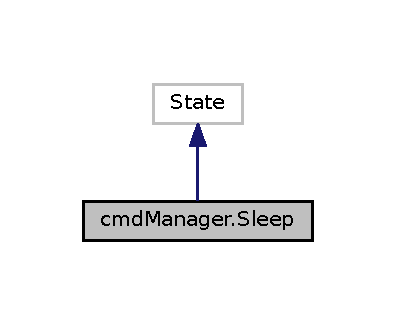
\includegraphics[width=190pt]{classcmdManager_1_1Sleep__inherit__graph}
\end{center}
\end{figure}


Collaboration diagram for cmd\+Manager.\+Sleep\+:
\nopagebreak
\begin{figure}[H]
\begin{center}
\leavevmode
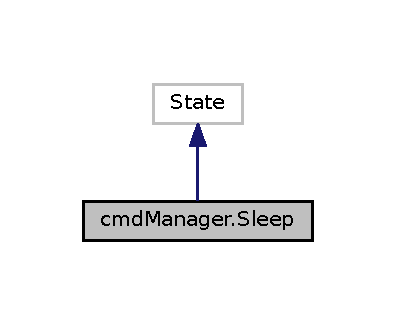
\includegraphics[width=190pt]{classcmdManager_1_1Sleep__coll__graph}
\end{center}
\end{figure}
\subsection*{Public Member Functions}
\begin{DoxyCompactItemize}
\item 
def \hyperlink{classcmdManager_1_1Sleep_ad60663dd525a5d09fc4b558d452aa2b3}{\+\_\+\+\_\+init\+\_\+\+\_\+} (self)
\item 
def \hyperlink{classcmdManager_1_1Sleep_a071852b6496ea38cff32c00186ebc0f6}{execute} (self, userdata)
\end{DoxyCompactItemize}
\subsection*{Public Attributes}
\begin{DoxyCompactItemize}
\item 
\hyperlink{classcmdManager_1_1Sleep_a0b3670d1b3a8cbbeb03935273320b858}{rate}
\end{DoxyCompactItemize}


\subsection{Detailed Description}
\begin{DoxyVerb}Class which define the SLEEP state of the FSM. In this state the robot go to the home position and sleep randomly, after that
the FSM return to NORMAL state\end{DoxyVerb}
 

\subsection{Constructor \& Destructor Documentation}
\index{cmd\+Manager\+::\+Sleep@{cmd\+Manager\+::\+Sleep}!\+\_\+\+\_\+init\+\_\+\+\_\+@{\+\_\+\+\_\+init\+\_\+\+\_\+}}
\index{\+\_\+\+\_\+init\+\_\+\+\_\+@{\+\_\+\+\_\+init\+\_\+\+\_\+}!cmd\+Manager\+::\+Sleep@{cmd\+Manager\+::\+Sleep}}
\subsubsection[{\texorpdfstring{\+\_\+\+\_\+init\+\_\+\+\_\+(self)}{__init__(self)}}]{\setlength{\rightskip}{0pt plus 5cm}def cmd\+Manager.\+Sleep.\+\_\+\+\_\+init\+\_\+\+\_\+ (
\begin{DoxyParamCaption}
\item[{}]{self}
\end{DoxyParamCaption}
)}\hypertarget{classcmdManager_1_1Sleep_ad60663dd525a5d09fc4b558d452aa2b3}{}\label{classcmdManager_1_1Sleep_ad60663dd525a5d09fc4b558d452aa2b3}


\subsection{Member Function Documentation}
\index{cmd\+Manager\+::\+Sleep@{cmd\+Manager\+::\+Sleep}!execute@{execute}}
\index{execute@{execute}!cmd\+Manager\+::\+Sleep@{cmd\+Manager\+::\+Sleep}}
\subsubsection[{\texorpdfstring{execute(self, userdata)}{execute(self, userdata)}}]{\setlength{\rightskip}{0pt plus 5cm}def cmd\+Manager.\+Sleep.\+execute (
\begin{DoxyParamCaption}
\item[{}]{self, }
\item[{}]{userdata}
\end{DoxyParamCaption}
)}\hypertarget{classcmdManager_1_1Sleep_a071852b6496ea38cff32c00186ebc0f6}{}\label{classcmdManager_1_1Sleep_a071852b6496ea38cff32c00186ebc0f6}


\subsection{Member Data Documentation}
\index{cmd\+Manager\+::\+Sleep@{cmd\+Manager\+::\+Sleep}!rate@{rate}}
\index{rate@{rate}!cmd\+Manager\+::\+Sleep@{cmd\+Manager\+::\+Sleep}}
\subsubsection[{\texorpdfstring{rate}{rate}}]{\setlength{\rightskip}{0pt plus 5cm}cmd\+Manager.\+Sleep.\+rate}\hypertarget{classcmdManager_1_1Sleep_a0b3670d1b3a8cbbeb03935273320b858}{}\label{classcmdManager_1_1Sleep_a0b3670d1b3a8cbbeb03935273320b858}


The documentation for this class was generated from the following file\+:\begin{DoxyCompactItemize}
\item 
/root/\+Desktop/catkin\+\_\+ws/src/exp\+\_\+assignment3/scripts/\hyperlink{cmdManager_8py}{cmd\+Manager.\+py}\end{DoxyCompactItemize}

\hypertarget{classcmdManager_1_1Track}{}\section{cmd\+Manager.\+Track Class Reference}
\label{classcmdManager_1_1Track}\index{cmd\+Manager.\+Track@{cmd\+Manager.\+Track}}


Inheritance diagram for cmd\+Manager.\+Track\+:
\nopagebreak
\begin{figure}[H]
\begin{center}
\leavevmode
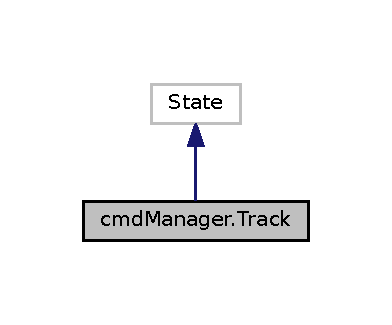
\includegraphics[width=188pt]{classcmdManager_1_1Track__inherit__graph}
\end{center}
\end{figure}


Collaboration diagram for cmd\+Manager.\+Track\+:
\nopagebreak
\begin{figure}[H]
\begin{center}
\leavevmode
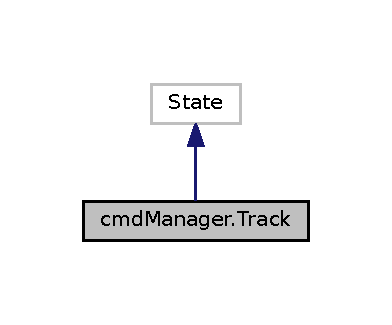
\includegraphics[width=188pt]{classcmdManager_1_1Track__coll__graph}
\end{center}
\end{figure}
\subsection*{Public Member Functions}
\begin{DoxyCompactItemize}
\item 
def \hyperlink{classcmdManager_1_1Track_a796dff8932a4e8e62b32f04b4f8481b6}{\+\_\+\+\_\+init\+\_\+\+\_\+} (self)
\item 
def \hyperlink{classcmdManager_1_1Track_ac3ae09cfd05e6d1f870422e0a8052acd}{execute} (self, userdata)
\end{DoxyCompactItemize}


\subsection{Detailed Description}
\begin{DoxyVerb}Class which define the TRACK stat of the FSM. Inside this state is initialized the client to the tracking action server
(implemented in trackingBall.py) which make the request of track the previuosly detected ball.\end{DoxyVerb}
 

\subsection{Constructor \& Destructor Documentation}
\index{cmd\+Manager\+::\+Track@{cmd\+Manager\+::\+Track}!\+\_\+\+\_\+init\+\_\+\+\_\+@{\+\_\+\+\_\+init\+\_\+\+\_\+}}
\index{\+\_\+\+\_\+init\+\_\+\+\_\+@{\+\_\+\+\_\+init\+\_\+\+\_\+}!cmd\+Manager\+::\+Track@{cmd\+Manager\+::\+Track}}
\subsubsection[{\texorpdfstring{\+\_\+\+\_\+init\+\_\+\+\_\+(self)}{__init__(self)}}]{\setlength{\rightskip}{0pt plus 5cm}def cmd\+Manager.\+Track.\+\_\+\+\_\+init\+\_\+\+\_\+ (
\begin{DoxyParamCaption}
\item[{}]{self}
\end{DoxyParamCaption}
)}\hypertarget{classcmdManager_1_1Track_a796dff8932a4e8e62b32f04b4f8481b6}{}\label{classcmdManager_1_1Track_a796dff8932a4e8e62b32f04b4f8481b6}


\subsection{Member Function Documentation}
\index{cmd\+Manager\+::\+Track@{cmd\+Manager\+::\+Track}!execute@{execute}}
\index{execute@{execute}!cmd\+Manager\+::\+Track@{cmd\+Manager\+::\+Track}}
\subsubsection[{\texorpdfstring{execute(self, userdata)}{execute(self, userdata)}}]{\setlength{\rightskip}{0pt plus 5cm}def cmd\+Manager.\+Track.\+execute (
\begin{DoxyParamCaption}
\item[{}]{self, }
\item[{}]{userdata}
\end{DoxyParamCaption}
)}\hypertarget{classcmdManager_1_1Track_ac3ae09cfd05e6d1f870422e0a8052acd}{}\label{classcmdManager_1_1Track_ac3ae09cfd05e6d1f870422e0a8052acd}


The documentation for this class was generated from the following file\+:\begin{DoxyCompactItemize}
\item 
/root/\+Desktop/catkin\+\_\+ws/src/exp\+\_\+assignment3/scripts/\hyperlink{cmdManager_8py}{cmd\+Manager.\+py}\end{DoxyCompactItemize}

\hypertarget{classtrackingBall_1_1Tracking}{}\section{tracking\+Ball.\+Tracking Class Reference}
\label{classtrackingBall_1_1Tracking}\index{tracking\+Ball.\+Tracking@{tracking\+Ball.\+Tracking}}


Class used for tracking the balls detected by ball\+Detect.\+py.  




Inheritance diagram for tracking\+Ball.\+Tracking\+:\nopagebreak
\begin{figure}[H]
\begin{center}
\leavevmode
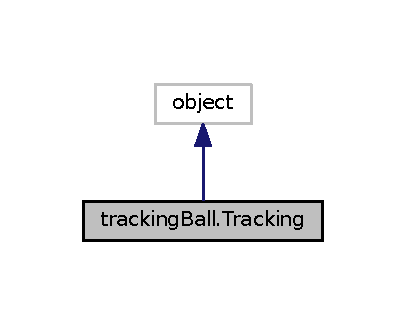
\includegraphics[width=195pt]{classtrackingBall_1_1Tracking__inherit__graph}
\end{center}
\end{figure}


Collaboration diagram for tracking\+Ball.\+Tracking\+:\nopagebreak
\begin{figure}[H]
\begin{center}
\leavevmode
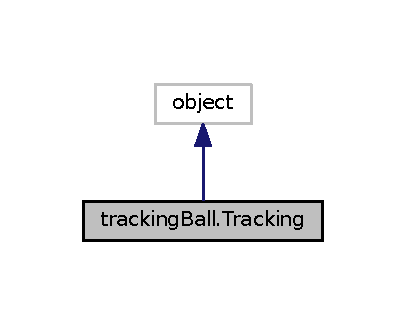
\includegraphics[width=195pt]{classtrackingBall_1_1Tracking__coll__graph}
\end{center}
\end{figure}
\subsection*{Public Member Functions}
\begin{DoxyCompactItemize}
\item 
def \hyperlink{classtrackingBall_1_1Tracking_afac83c606a2539723c13ed9d08385729}{\+\_\+\+\_\+init\+\_\+\+\_\+} (self, name)
\item 
def \hyperlink{classtrackingBall_1_1Tracking_ae942d974bcf15ea113ddbdb845b93914}{odom\+\_\+clbk} (self, msg)
\begin{DoxyCompactList}\small\item\em Callbak to the /odom subscriber (update pose and position of the robot) \end{DoxyCompactList}\item 
def \hyperlink{classtrackingBall_1_1Tracking_a1d98727a3d632e7e5ae973cb3417837a}{go\+\_\+to\+\_\+ball} (self, ros\+\_\+image)
\begin{DoxyCompactList}\small\item\em Callback of the \char`\"{}camera1/image\+\_\+raw/compressed\char`\"{} subscriber, allows the robot to move towards the ball. \end{DoxyCompactList}\item 
def \hyperlink{classtrackingBall_1_1Tracking_aa69933a4bd0f18dd53c4d2db71c0d691}{avoid\+\_\+obstacle} (self, msg)
\begin{DoxyCompactList}\small\item\em Callback of the subscriber to the laser scan, is used for implement a simple bug algorithm for obstacle avoidance during tracking. \end{DoxyCompactList}\item 
def \hyperlink{classtrackingBall_1_1Tracking_aab79d6fd3ebcc645ac180b827ab8a4ad}{track} (self, goal)
\begin{DoxyCompactList}\small\item\em A\+C\+T\+I\+ON S\+E\+R\+V\+ER F\+U\+N\+C\+T\+I\+ON. \end{DoxyCompactList}\end{DoxyCompactItemize}
\subsection*{Public Attributes}
\begin{DoxyCompactItemize}
\item 
\hyperlink{classtrackingBall_1_1Tracking_a6b17306fa008c6665ff8a5798ee27ba8}{action\+\_\+name}
\begin{DoxyCompactList}\small\item\em N\+A\+ME OF T\+HE S\+E\+R\+V\+ER. \end{DoxyCompactList}\item 
\hyperlink{classtrackingBall_1_1Tracking_a46586a7a898c757afcff8d89a7b55d77}{act\+\_\+s}
\item 
\hyperlink{classtrackingBall_1_1Tracking_a9d40ea04aba08e244a8edf175d659229}{feedback}
\item 
\hyperlink{classtrackingBall_1_1Tracking_abe3eb1a78c5f9464274125a664c694b9}{result}
\item 
\hyperlink{classtrackingBall_1_1Tracking_af4673dff355192ccd7cbd4e3676ef618}{lidar\+\_\+regions}
\begin{DoxyCompactList}\small\item\em D\+I\+CT F\+OR O\+B\+S\+T\+A\+C\+LE A\+V\+O\+I\+D\+A\+N\+CE A\+L\+G\+O\+R\+I\+T\+HM (store the regions of the lidar for be able to localize the obstacle w.\+r.\+t. \end{DoxyCompactList}\item 
\hyperlink{classtrackingBall_1_1Tracking_aadfc96c3a6be143bb62858a7ac2fc840}{A\+C\+K\+\_\+\+P\+O\+S\+I\+T\+I\+VO}
\begin{DoxyCompactList}\small\item\em B\+O\+O\+L\+E\+AN OF A\+C\+K\+N\+O\+W\+L\+E\+D\+G\+M\+E\+NT P\+O\+S\+I\+T\+I\+VO IF T\+HE M\+I\+S\+S\+I\+ON IS F\+I\+N\+I\+SH C\+O\+R\+R\+E\+C\+T\+LY. \end{DoxyCompactList}\item 
\hyperlink{classtrackingBall_1_1Tracking_a89db2b56bfd79bbbac1fd1af937e25f8}{lost\+\_\+ball\+\_\+counter}
\begin{DoxyCompactList}\small\item\em C\+O\+U\+N\+T\+ER F\+OR M\+O\+N\+I\+T\+OR T\+HE T\+R\+A\+C\+K\+I\+NG W\+H\+I\+LE T\+HE B\+A\+LL IS L\+O\+ST. \end{DoxyCompactList}\item 
\hyperlink{classtrackingBall_1_1Tracking_a7ce6a966db6cba83ba1ade3c1e7408a1}{A\+C\+K\+\_\+\+N\+E\+G\+A\+T\+I\+VO}
\begin{DoxyCompactList}\small\item\em Subscriber to camera topic, after receiving image start the tracking. \end{DoxyCompactList}\item 
\hyperlink{classtrackingBall_1_1Tracking_a9216a69022a6756b653d59834bb46de3}{radius}
\begin{DoxyCompactList}\small\item\em R\+A\+D\+I\+US OF T\+HE B\+A\+LL IN T\+HE I\+M\+A\+GE. \end{DoxyCompactList}\item 
\hyperlink{classtrackingBall_1_1Tracking_aec612c6502c0a334f67d8b32e7b77b62}{vel\+\_\+publisher}
\begin{DoxyCompactList}\small\item\em I\+N\+I\+T\+I\+A\+L\+I\+Z\+A\+T\+I\+ON OF T\+HE V\+E\+L\+O\+C\+I\+TY P\+U\+B\+L\+I\+S\+H\+ER TO T\+HE W\+H\+E\+E\+LS. \end{DoxyCompactList}\item 
\hyperlink{classtrackingBall_1_1Tracking_a8698f440e6e3e4b1b785cab162794b61}{position}
\begin{DoxyCompactList}\small\item\em I\+N\+IT R\+O\+B\+OT P\+O\+S\+I\+T\+I\+ON. \end{DoxyCompactList}\item 
\hyperlink{classtrackingBall_1_1Tracking_af3d46e4a3b61c4cc2841cfdd6e02c459}{pose}
\begin{DoxyCompactList}\small\item\em I\+N\+IT R\+O\+B\+OT P\+O\+SE. \end{DoxyCompactList}\item 
\hyperlink{classtrackingBall_1_1Tracking_a684292f4752cf04f4aeb3baf84e0b155}{sigma\+Linear}
\begin{DoxyCompactList}\small\item\em P\+A\+R\+A\+M\+E\+T\+ER F\+OR C\+O\+R\+R\+E\+CT L\+I\+N\+E\+AR V\+E\+L\+O\+C\+I\+TY D\+U\+R\+I\+NG T\+R\+A\+C\+K\+I\+NG (for smooth movements) \end{DoxyCompactList}\item 
\hyperlink{classtrackingBall_1_1Tracking_abcf19d205ec149c4f87a2c3b43fa242e}{sigma\+Angular}
\begin{DoxyCompactList}\small\item\em P\+A\+R\+A\+M\+E\+T\+ER F\+OR C\+O\+R\+R\+E\+CT A\+N\+G\+U\+L\+AR V\+E\+L\+O\+C\+I\+TY D\+U\+R\+I\+NG T\+R\+A\+C\+K\+I\+NG (for smooth movements) \end{DoxyCompactList}\item 
\hyperlink{classtrackingBall_1_1Tracking_aa5264f9fd30dcb6818c64175c9aa9a88}{color}
\begin{DoxyCompactList}\small\item\em Reduce noise. \end{DoxyCompactList}\end{DoxyCompactItemize}


\subsection{Detailed Description}
Class used for tracking the balls detected by ball\+Detect.\+py. 

After receiving the request from the client (Cmd\+\_\+\+Manager\+\_\+\+Node) the script start to track the ball of the color sended by the client. It also save the robot position subscribing to /odom topic for store the room position. Sice during the tracking the move\+\_\+base action is aborted, it\textquotesingle{}s also implemented a simple obstacle avoidance using the \char`\"{}bug algorithm\char`\"{} for prevent the robot collide with obstacle during the approaching to the ball. 

\subsection{Constructor \& Destructor Documentation}
\index{tracking\+Ball\+::\+Tracking@{tracking\+Ball\+::\+Tracking}!\+\_\+\+\_\+init\+\_\+\+\_\+@{\+\_\+\+\_\+init\+\_\+\+\_\+}}
\index{\+\_\+\+\_\+init\+\_\+\+\_\+@{\+\_\+\+\_\+init\+\_\+\+\_\+}!tracking\+Ball\+::\+Tracking@{tracking\+Ball\+::\+Tracking}}
\subsubsection[{\texorpdfstring{\+\_\+\+\_\+init\+\_\+\+\_\+(self, name)}{__init__(self, name)}}]{\setlength{\rightskip}{0pt plus 5cm}def tracking\+Ball.\+Tracking.\+\_\+\+\_\+init\+\_\+\+\_\+ (
\begin{DoxyParamCaption}
\item[{}]{self, }
\item[{}]{name}
\end{DoxyParamCaption}
)}\hypertarget{classtrackingBall_1_1Tracking_afac83c606a2539723c13ed9d08385729}{}\label{classtrackingBall_1_1Tracking_afac83c606a2539723c13ed9d08385729}


\subsection{Member Function Documentation}
\index{tracking\+Ball\+::\+Tracking@{tracking\+Ball\+::\+Tracking}!avoid\+\_\+obstacle@{avoid\+\_\+obstacle}}
\index{avoid\+\_\+obstacle@{avoid\+\_\+obstacle}!tracking\+Ball\+::\+Tracking@{tracking\+Ball\+::\+Tracking}}
\subsubsection[{\texorpdfstring{avoid\+\_\+obstacle(self, msg)}{avoid_obstacle(self, msg)}}]{\setlength{\rightskip}{0pt plus 5cm}def tracking\+Ball.\+Tracking.\+avoid\+\_\+obstacle (
\begin{DoxyParamCaption}
\item[{}]{self, }
\item[{}]{msg}
\end{DoxyParamCaption}
)}\hypertarget{classtrackingBall_1_1Tracking_aa69933a4bd0f18dd53c4d2db71c0d691}{}\label{classtrackingBall_1_1Tracking_aa69933a4bd0f18dd53c4d2db71c0d691}


Callback of the subscriber to the laser scan, is used for implement a simple bug algorithm for obstacle avoidance during tracking. 


\begin{DoxyParams}{Parameters}
{\em msg} & Laser\+Scan message --$>$ distance from the obstacle \\
\hline
\end{DoxyParams}
\index{tracking\+Ball\+::\+Tracking@{tracking\+Ball\+::\+Tracking}!go\+\_\+to\+\_\+ball@{go\+\_\+to\+\_\+ball}}
\index{go\+\_\+to\+\_\+ball@{go\+\_\+to\+\_\+ball}!tracking\+Ball\+::\+Tracking@{tracking\+Ball\+::\+Tracking}}
\subsubsection[{\texorpdfstring{go\+\_\+to\+\_\+ball(self, ros\+\_\+image)}{go_to_ball(self, ros_image)}}]{\setlength{\rightskip}{0pt plus 5cm}def tracking\+Ball.\+Tracking.\+go\+\_\+to\+\_\+ball (
\begin{DoxyParamCaption}
\item[{}]{self, }
\item[{}]{ros\+\_\+image}
\end{DoxyParamCaption}
)}\hypertarget{classtrackingBall_1_1Tracking_a1d98727a3d632e7e5ae973cb3417837a}{}\label{classtrackingBall_1_1Tracking_a1d98727a3d632e7e5ae973cb3417837a}


Callback of the \char`\"{}camera1/image\+\_\+raw/compressed\char`\"{} subscriber, allows the robot to move towards the ball. 

\index{tracking\+Ball\+::\+Tracking@{tracking\+Ball\+::\+Tracking}!odom\+\_\+clbk@{odom\+\_\+clbk}}
\index{odom\+\_\+clbk@{odom\+\_\+clbk}!tracking\+Ball\+::\+Tracking@{tracking\+Ball\+::\+Tracking}}
\subsubsection[{\texorpdfstring{odom\+\_\+clbk(self, msg)}{odom_clbk(self, msg)}}]{\setlength{\rightskip}{0pt plus 5cm}def tracking\+Ball.\+Tracking.\+odom\+\_\+clbk (
\begin{DoxyParamCaption}
\item[{}]{self, }
\item[{}]{msg}
\end{DoxyParamCaption}
)}\hypertarget{classtrackingBall_1_1Tracking_ae942d974bcf15ea113ddbdb845b93914}{}\label{classtrackingBall_1_1Tracking_ae942d974bcf15ea113ddbdb845b93914}


Callbak to the /odom subscriber (update pose and position of the robot) 

\index{tracking\+Ball\+::\+Tracking@{tracking\+Ball\+::\+Tracking}!track@{track}}
\index{track@{track}!tracking\+Ball\+::\+Tracking@{tracking\+Ball\+::\+Tracking}}
\subsubsection[{\texorpdfstring{track(self, goal)}{track(self, goal)}}]{\setlength{\rightskip}{0pt plus 5cm}def tracking\+Ball.\+Tracking.\+track (
\begin{DoxyParamCaption}
\item[{}]{self, }
\item[{}]{goal}
\end{DoxyParamCaption}
)}\hypertarget{classtrackingBall_1_1Tracking_aab79d6fd3ebcc645ac180b827ab8a4ad}{}\label{classtrackingBall_1_1Tracking_aab79d6fd3ebcc645ac180b827ab8a4ad}


A\+C\+T\+I\+ON S\+E\+R\+V\+ER F\+U\+N\+C\+T\+I\+ON. 


\begin{DoxyParams}{Parameters}
{\em goal} & contain the color of the ball to track. \\
\hline
\end{DoxyParams}


\subsection{Member Data Documentation}
\index{tracking\+Ball\+::\+Tracking@{tracking\+Ball\+::\+Tracking}!A\+C\+K\+\_\+\+N\+E\+G\+A\+T\+I\+VO@{A\+C\+K\+\_\+\+N\+E\+G\+A\+T\+I\+VO}}
\index{A\+C\+K\+\_\+\+N\+E\+G\+A\+T\+I\+VO@{A\+C\+K\+\_\+\+N\+E\+G\+A\+T\+I\+VO}!tracking\+Ball\+::\+Tracking@{tracking\+Ball\+::\+Tracking}}
\subsubsection[{\texorpdfstring{A\+C\+K\+\_\+\+N\+E\+G\+A\+T\+I\+VO}{ACK_NEGATIVO}}]{\setlength{\rightskip}{0pt plus 5cm}tracking\+Ball.\+Tracking.\+A\+C\+K\+\_\+\+N\+E\+G\+A\+T\+I\+VO}\hypertarget{classtrackingBall_1_1Tracking_a7ce6a966db6cba83ba1ade3c1e7408a1}{}\label{classtrackingBall_1_1Tracking_a7ce6a966db6cba83ba1ade3c1e7408a1}


Subscriber to camera topic, after receiving image start the tracking. 

Subscriber to Laser Scan topic, for implement ostacle avoidance. \index{tracking\+Ball\+::\+Tracking@{tracking\+Ball\+::\+Tracking}!A\+C\+K\+\_\+\+P\+O\+S\+I\+T\+I\+VO@{A\+C\+K\+\_\+\+P\+O\+S\+I\+T\+I\+VO}}
\index{A\+C\+K\+\_\+\+P\+O\+S\+I\+T\+I\+VO@{A\+C\+K\+\_\+\+P\+O\+S\+I\+T\+I\+VO}!tracking\+Ball\+::\+Tracking@{tracking\+Ball\+::\+Tracking}}
\subsubsection[{\texorpdfstring{A\+C\+K\+\_\+\+P\+O\+S\+I\+T\+I\+VO}{ACK_POSITIVO}}]{\setlength{\rightskip}{0pt plus 5cm}tracking\+Ball.\+Tracking.\+A\+C\+K\+\_\+\+P\+O\+S\+I\+T\+I\+VO}\hypertarget{classtrackingBall_1_1Tracking_aadfc96c3a6be143bb62858a7ac2fc840}{}\label{classtrackingBall_1_1Tracking_aadfc96c3a6be143bb62858a7ac2fc840}


B\+O\+O\+L\+E\+AN OF A\+C\+K\+N\+O\+W\+L\+E\+D\+G\+M\+E\+NT P\+O\+S\+I\+T\+I\+VO IF T\+HE M\+I\+S\+S\+I\+ON IS F\+I\+N\+I\+SH C\+O\+R\+R\+E\+C\+T\+LY. 

\index{tracking\+Ball\+::\+Tracking@{tracking\+Ball\+::\+Tracking}!act\+\_\+s@{act\+\_\+s}}
\index{act\+\_\+s@{act\+\_\+s}!tracking\+Ball\+::\+Tracking@{tracking\+Ball\+::\+Tracking}}
\subsubsection[{\texorpdfstring{act\+\_\+s}{act_s}}]{\setlength{\rightskip}{0pt plus 5cm}tracking\+Ball.\+Tracking.\+act\+\_\+s}\hypertarget{classtrackingBall_1_1Tracking_a46586a7a898c757afcff8d89a7b55d77}{}\label{classtrackingBall_1_1Tracking_a46586a7a898c757afcff8d89a7b55d77}
\index{tracking\+Ball\+::\+Tracking@{tracking\+Ball\+::\+Tracking}!action\+\_\+name@{action\+\_\+name}}
\index{action\+\_\+name@{action\+\_\+name}!tracking\+Ball\+::\+Tracking@{tracking\+Ball\+::\+Tracking}}
\subsubsection[{\texorpdfstring{action\+\_\+name}{action_name}}]{\setlength{\rightskip}{0pt plus 5cm}tracking\+Ball.\+Tracking.\+action\+\_\+name}\hypertarget{classtrackingBall_1_1Tracking_a6b17306fa008c6665ff8a5798ee27ba8}{}\label{classtrackingBall_1_1Tracking_a6b17306fa008c6665ff8a5798ee27ba8}


N\+A\+ME OF T\+HE S\+E\+R\+V\+ER. 

\index{tracking\+Ball\+::\+Tracking@{tracking\+Ball\+::\+Tracking}!color@{color}}
\index{color@{color}!tracking\+Ball\+::\+Tracking@{tracking\+Ball\+::\+Tracking}}
\subsubsection[{\texorpdfstring{color}{color}}]{\setlength{\rightskip}{0pt plus 5cm}tracking\+Ball.\+Tracking.\+color}\hypertarget{classtrackingBall_1_1Tracking_aa5264f9fd30dcb6818c64175c9aa9a88}{}\label{classtrackingBall_1_1Tracking_aa5264f9fd30dcb6818c64175c9aa9a88}


Reduce noise. 


\begin{DoxyParams}{Parameters}
{\em image\+\_\+np} & (decompresed image and converted to C\+V2) Conversion to hsv \\
\hline
\end{DoxyParams}
\index{tracking\+Ball\+::\+Tracking@{tracking\+Ball\+::\+Tracking}!feedback@{feedback}}
\index{feedback@{feedback}!tracking\+Ball\+::\+Tracking@{tracking\+Ball\+::\+Tracking}}
\subsubsection[{\texorpdfstring{feedback}{feedback}}]{\setlength{\rightskip}{0pt plus 5cm}tracking\+Ball.\+Tracking.\+feedback}\hypertarget{classtrackingBall_1_1Tracking_a9d40ea04aba08e244a8edf175d659229}{}\label{classtrackingBall_1_1Tracking_a9d40ea04aba08e244a8edf175d659229}
\index{tracking\+Ball\+::\+Tracking@{tracking\+Ball\+::\+Tracking}!lidar\+\_\+regions@{lidar\+\_\+regions}}
\index{lidar\+\_\+regions@{lidar\+\_\+regions}!tracking\+Ball\+::\+Tracking@{tracking\+Ball\+::\+Tracking}}
\subsubsection[{\texorpdfstring{lidar\+\_\+regions}{lidar_regions}}]{\setlength{\rightskip}{0pt plus 5cm}tracking\+Ball.\+Tracking.\+lidar\+\_\+regions}\hypertarget{classtrackingBall_1_1Tracking_af4673dff355192ccd7cbd4e3676ef618}{}\label{classtrackingBall_1_1Tracking_af4673dff355192ccd7cbd4e3676ef618}


D\+I\+CT F\+OR O\+B\+S\+T\+A\+C\+LE A\+V\+O\+I\+D\+A\+N\+CE A\+L\+G\+O\+R\+I\+T\+HM (store the regions of the lidar for be able to localize the obstacle w.\+r.\+t. 

the robot) \index{tracking\+Ball\+::\+Tracking@{tracking\+Ball\+::\+Tracking}!lost\+\_\+ball\+\_\+counter@{lost\+\_\+ball\+\_\+counter}}
\index{lost\+\_\+ball\+\_\+counter@{lost\+\_\+ball\+\_\+counter}!tracking\+Ball\+::\+Tracking@{tracking\+Ball\+::\+Tracking}}
\subsubsection[{\texorpdfstring{lost\+\_\+ball\+\_\+counter}{lost_ball_counter}}]{\setlength{\rightskip}{0pt plus 5cm}tracking\+Ball.\+Tracking.\+lost\+\_\+ball\+\_\+counter}\hypertarget{classtrackingBall_1_1Tracking_a89db2b56bfd79bbbac1fd1af937e25f8}{}\label{classtrackingBall_1_1Tracking_a89db2b56bfd79bbbac1fd1af937e25f8}


C\+O\+U\+N\+T\+ER F\+OR M\+O\+N\+I\+T\+OR T\+HE T\+R\+A\+C\+K\+I\+NG W\+H\+I\+LE T\+HE B\+A\+LL IS L\+O\+ST. 

\index{tracking\+Ball\+::\+Tracking@{tracking\+Ball\+::\+Tracking}!pose@{pose}}
\index{pose@{pose}!tracking\+Ball\+::\+Tracking@{tracking\+Ball\+::\+Tracking}}
\subsubsection[{\texorpdfstring{pose}{pose}}]{\setlength{\rightskip}{0pt plus 5cm}tracking\+Ball.\+Tracking.\+pose}\hypertarget{classtrackingBall_1_1Tracking_af3d46e4a3b61c4cc2841cfdd6e02c459}{}\label{classtrackingBall_1_1Tracking_af3d46e4a3b61c4cc2841cfdd6e02c459}


I\+N\+IT R\+O\+B\+OT P\+O\+SE. 

\index{tracking\+Ball\+::\+Tracking@{tracking\+Ball\+::\+Tracking}!position@{position}}
\index{position@{position}!tracking\+Ball\+::\+Tracking@{tracking\+Ball\+::\+Tracking}}
\subsubsection[{\texorpdfstring{position}{position}}]{\setlength{\rightskip}{0pt plus 5cm}tracking\+Ball.\+Tracking.\+position}\hypertarget{classtrackingBall_1_1Tracking_a8698f440e6e3e4b1b785cab162794b61}{}\label{classtrackingBall_1_1Tracking_a8698f440e6e3e4b1b785cab162794b61}


I\+N\+IT R\+O\+B\+OT P\+O\+S\+I\+T\+I\+ON. 

\index{tracking\+Ball\+::\+Tracking@{tracking\+Ball\+::\+Tracking}!radius@{radius}}
\index{radius@{radius}!tracking\+Ball\+::\+Tracking@{tracking\+Ball\+::\+Tracking}}
\subsubsection[{\texorpdfstring{radius}{radius}}]{\setlength{\rightskip}{0pt plus 5cm}tracking\+Ball.\+Tracking.\+radius}\hypertarget{classtrackingBall_1_1Tracking_a9216a69022a6756b653d59834bb46de3}{}\label{classtrackingBall_1_1Tracking_a9216a69022a6756b653d59834bb46de3}


R\+A\+D\+I\+US OF T\+HE B\+A\+LL IN T\+HE I\+M\+A\+GE. 

\index{tracking\+Ball\+::\+Tracking@{tracking\+Ball\+::\+Tracking}!result@{result}}
\index{result@{result}!tracking\+Ball\+::\+Tracking@{tracking\+Ball\+::\+Tracking}}
\subsubsection[{\texorpdfstring{result}{result}}]{\setlength{\rightskip}{0pt plus 5cm}tracking\+Ball.\+Tracking.\+result}\hypertarget{classtrackingBall_1_1Tracking_abe3eb1a78c5f9464274125a664c694b9}{}\label{classtrackingBall_1_1Tracking_abe3eb1a78c5f9464274125a664c694b9}
\index{tracking\+Ball\+::\+Tracking@{tracking\+Ball\+::\+Tracking}!sigma\+Angular@{sigma\+Angular}}
\index{sigma\+Angular@{sigma\+Angular}!tracking\+Ball\+::\+Tracking@{tracking\+Ball\+::\+Tracking}}
\subsubsection[{\texorpdfstring{sigma\+Angular}{sigmaAngular}}]{\setlength{\rightskip}{0pt plus 5cm}tracking\+Ball.\+Tracking.\+sigma\+Angular}\hypertarget{classtrackingBall_1_1Tracking_abcf19d205ec149c4f87a2c3b43fa242e}{}\label{classtrackingBall_1_1Tracking_abcf19d205ec149c4f87a2c3b43fa242e}


P\+A\+R\+A\+M\+E\+T\+ER F\+OR C\+O\+R\+R\+E\+CT A\+N\+G\+U\+L\+AR V\+E\+L\+O\+C\+I\+TY D\+U\+R\+I\+NG T\+R\+A\+C\+K\+I\+NG (for smooth movements) 

\index{tracking\+Ball\+::\+Tracking@{tracking\+Ball\+::\+Tracking}!sigma\+Linear@{sigma\+Linear}}
\index{sigma\+Linear@{sigma\+Linear}!tracking\+Ball\+::\+Tracking@{tracking\+Ball\+::\+Tracking}}
\subsubsection[{\texorpdfstring{sigma\+Linear}{sigmaLinear}}]{\setlength{\rightskip}{0pt plus 5cm}tracking\+Ball.\+Tracking.\+sigma\+Linear}\hypertarget{classtrackingBall_1_1Tracking_a684292f4752cf04f4aeb3baf84e0b155}{}\label{classtrackingBall_1_1Tracking_a684292f4752cf04f4aeb3baf84e0b155}


P\+A\+R\+A\+M\+E\+T\+ER F\+OR C\+O\+R\+R\+E\+CT L\+I\+N\+E\+AR V\+E\+L\+O\+C\+I\+TY D\+U\+R\+I\+NG T\+R\+A\+C\+K\+I\+NG (for smooth movements) 

\index{tracking\+Ball\+::\+Tracking@{tracking\+Ball\+::\+Tracking}!vel\+\_\+publisher@{vel\+\_\+publisher}}
\index{vel\+\_\+publisher@{vel\+\_\+publisher}!tracking\+Ball\+::\+Tracking@{tracking\+Ball\+::\+Tracking}}
\subsubsection[{\texorpdfstring{vel\+\_\+publisher}{vel_publisher}}]{\setlength{\rightskip}{0pt plus 5cm}tracking\+Ball.\+Tracking.\+vel\+\_\+publisher}\hypertarget{classtrackingBall_1_1Tracking_aec612c6502c0a334f67d8b32e7b77b62}{}\label{classtrackingBall_1_1Tracking_aec612c6502c0a334f67d8b32e7b77b62}


I\+N\+I\+T\+I\+A\+L\+I\+Z\+A\+T\+I\+ON OF T\+HE V\+E\+L\+O\+C\+I\+TY P\+U\+B\+L\+I\+S\+H\+ER TO T\+HE W\+H\+E\+E\+LS. 

Subscriber to the odometry of the robot for update pose and position.

Publisher of the velocity commands for the robot. 

The documentation for this class was generated from the following file\+:\begin{DoxyCompactItemize}
\item 
/root/\+Desktop/catkin\+\_\+ws/src/exp\+\_\+assignment3/scripts/\hyperlink{trackingBall_8py}{tracking\+Ball.\+py}\end{DoxyCompactItemize}

\chapter{File Documentation}
\hypertarget{ballDetection_8py}{}\section{/root/\+Desktop/catkin\+\_\+ws/src/exp\+\_\+assignment3/scripts/ball\+Detection.py File Reference}
\label{ballDetection_8py}\index{/root/\+Desktop/catkin\+\_\+ws/src/exp\+\_\+assignment3/scripts/ball\+Detection.\+py@{/root/\+Desktop/catkin\+\_\+ws/src/exp\+\_\+assignment3/scripts/ball\+Detection.\+py}}
\subsection*{Classes}
\begin{DoxyCompactItemize}
\item 
class \hyperlink{classballDetection_1_1ballDetector}{ball\+Detection.\+ball\+Detector}
\begin{DoxyCompactList}\small\item\em Class which define the color detection algorithm used which run in a node on his own. \end{DoxyCompactList}\end{DoxyCompactItemize}
\subsection*{Namespaces}
\begin{DoxyCompactItemize}
\item 
 \hyperlink{namespaceballDetection}{ball\+Detection}
\end{DoxyCompactItemize}
\subsection*{Functions}
\begin{DoxyCompactItemize}
\item 
def \hyperlink{namespaceballDetection_af90d57b7d5fbbaa648ba3ba524d541dd}{ball\+Detection.\+detection\+State} (state, rd)
\begin{DoxyCompactList}\small\item\em This is the callback function of the subscriber to  topic, it receive a boolen which notify to start the detection or stop it. \end{DoxyCompactList}\item 
def \hyperlink{namespaceballDetection_a8193b8aef394c20f60fadbaeacdafdc0}{ball\+Detection.\+main} (args)
\end{DoxyCompactItemize}
\subsection*{Variables}
\begin{DoxyCompactItemize}
\item 
tuple \hyperlink{namespaceballDetection_a39a98090c55ec606030abf18d6820366}{ball\+Detection.\+black\+Lower} = (0, 0, 0)
\item 
tuple \hyperlink{namespaceballDetection_a23ab917df5c9f52915a32ec50221f14f}{ball\+Detection.\+black\+Upper} = (5,50,50)
\item 
tuple \hyperlink{namespaceballDetection_a92ef9da6121e329eb1703494c3104863}{ball\+Detection.\+red\+Lower} = (0, 50, 50)
\item 
tuple \hyperlink{namespaceballDetection_aa460677a3e1cdb2341aeba5fd17aa2b6}{ball\+Detection.\+red\+Upper} = (5, 255, 255)
\item 
tuple \hyperlink{namespaceballDetection_a13f45d6a550517a155e1b28fbb1e21b5}{ball\+Detection.\+yellow\+Lower} = (25, 50, 50)
\item 
tuple \hyperlink{namespaceballDetection_aaf6f118d96c2df97f6779017e31994af}{ball\+Detection.\+yellow\+Upper} = (35, 255, 255)
\item 
tuple \hyperlink{namespaceballDetection_a9baf8ab116194ae3b105440b2331765c}{ball\+Detection.\+green\+Lower} = (50, 50, 50)
\item 
tuple \hyperlink{namespaceballDetection_a1132c3cfcdb75ebb1e6ee6318c4caf2d}{ball\+Detection.\+green\+Upper} = (70, 255, 255)
\item 
tuple \hyperlink{namespaceballDetection_a7c95f76d92a79c2eba518529d4585fbe}{ball\+Detection.\+blue\+Lower} = (100, 50, 50)
\item 
tuple \hyperlink{namespaceballDetection_a32646e670c980662c55d776abcd8615e}{ball\+Detection.\+blue\+Upper} = (130, 255, 255)
\item 
tuple \hyperlink{namespaceballDetection_ac513c92adbc3a5f8325877d042cf28fb}{ball\+Detection.\+magenta\+Lower} = (125, 50, 50)
\item 
tuple \hyperlink{namespaceballDetection_a3d5c34f17eec8c6b35c650d34409cf6e}{ball\+Detection.\+magenta\+Upper} = (150, 255, 255)
\end{DoxyCompactItemize}

\hypertarget{cmdManager_8py}{}\section{/root/\+Desktop/catkin\+\_\+ws/src/exp\+\_\+assignment3/scripts/cmd\+Manager.py File Reference}
\label{cmdManager_8py}\index{/root/\+Desktop/catkin\+\_\+ws/src/exp\+\_\+assignment3/scripts/cmd\+Manager.\+py@{/root/\+Desktop/catkin\+\_\+ws/src/exp\+\_\+assignment3/scripts/cmd\+Manager.\+py}}
\subsection*{Classes}
\begin{DoxyCompactItemize}
\item 
class \hyperlink{classcmdManager_1_1Normal}{cmd\+Manager.\+Normal}
\item 
class \hyperlink{classcmdManager_1_1Sleep}{cmd\+Manager.\+Sleep}
\item 
class \hyperlink{classcmdManager_1_1Play}{cmd\+Manager.\+Play}
\item 
class \hyperlink{classcmdManager_1_1Find}{cmd\+Manager.\+Find}
\item 
class \hyperlink{classcmdManager_1_1Track}{cmd\+Manager.\+Track}
\end{DoxyCompactItemize}
\subsection*{Namespaces}
\begin{DoxyCompactItemize}
\item 
 \hyperlink{namespacecmdManager}{cmd\+Manager}
\end{DoxyCompactItemize}
\subsection*{Functions}
\begin{DoxyCompactItemize}
\item 
def \hyperlink{namespacecmdManager_a62a68181d751176538db8063d7b11987}{cmd\+Manager.\+detection\+\_\+routine} (color)
\begin{DoxyCompactList}\small\item\em Callback of the ball\+\_\+detection\+\_\+subscriber, is called any time a new colored ball is found, precisely a new color is given in input and then the function check if the color was already detected, if not the move\+\_\+base client is stopped for start the tracking. \end{DoxyCompactList}\item 
def \hyperlink{namespacecmdManager_a50ab72ebc575eb7032c50d17a6d592c6}{cmd\+Manager.\+U\+Icallback} (data)
\begin{DoxyCompactList}\small\item\em Callback of the human interface, each time a user command is received the function change the P\+L\+AY flag and the message is parsed. \end{DoxyCompactList}\item 
def \hyperlink{namespacecmdManager_ac53d2d1248b660039d5a90768ff3bd5e}{cmd\+Manager.\+go\+\_\+to} (x, y)
\begin{DoxyCompactList}\small\item\em Function which implement the navigation to given input position using the move\+\_\+base action server. \end{DoxyCompactList}\item 
def \hyperlink{namespacecmdManager_a3e64a5e295736776673178e6ff94d1e5}{cmd\+Manager.\+main} ()
\end{DoxyCompactItemize}
\subsection*{Variables}
\begin{DoxyCompactItemize}
\item 
\hyperlink{namespacecmdManager_ad1967c9cd71b2174a9b4c56d32f08fcc}{cmd\+Manager.\+client} = actionlib.\+Simple\+Action\+Client(\textquotesingle{}move\+\_\+base\textquotesingle{},Move\+Base\+Action)
\begin{DoxyCompactList}\small\item\em Initialized the client to the move\+\_\+base action server for moving the robot. \end{DoxyCompactList}\item 
\hyperlink{namespacecmdManager_a5f10b08efaeaad88cf34e075895f4d9d}{cmd\+Manager.\+R\+D\+\_\+pub} = rospy.\+Publisher(\textquotesingle{}detection\+\_\+state\textquotesingle{}, Bool, queue\+\_\+size=10)
\begin{DoxyCompactList}\small\item\em Initialized publisher of the detection state which is a boolean (active or not). \end{DoxyCompactList}\item 
\hyperlink{namespacecmdManager_a783b0ef84682af39dc9f2b8e828c4ad9}{cmd\+Manager.\+rooms} = Rooms()
\begin{DoxyCompactList}\small\item\em Initialized object of the class Rooms() for use the knowledge representation defined in \hyperlink{knowledgeRep_8py}{knowledge\+Rep.\+py}. \end{DoxyCompactList}\item 
dictionary \hyperlink{namespacecmdManager_a927e4211865b745599afe42e9e8d7c8e}{cmd\+Manager.\+ctrl\+\_\+var} = \{\char`\"{}P\+L\+AY\char`\"{} \+: False, \char`\"{}T\+A\+R\+G\+E\+T\+\_\+\+R\+O\+OM\char`\"{} \+: \char`\"{}None\char`\"{}, \char`\"{}N\+E\+W\+\_\+\+C\+O\+L\+OR\char`\"{} \+: \char`\"{}None\char`\"{}, \char`\"{}F\+I\+ND\char`\"{} \+: False\}
\begin{DoxyCompactList}\small\item\em Dictionary that store important control variables and flags. \end{DoxyCompactList}\end{DoxyCompactItemize}

\hypertarget{humanInterface_8py}{}\section{/root/\+Desktop/catkin\+\_\+ws/src/exp\+\_\+assignment3/scripts/human\+Interface.py File Reference}
\label{humanInterface_8py}\index{/root/\+Desktop/catkin\+\_\+ws/src/exp\+\_\+assignment3/scripts/human\+Interface.\+py@{/root/\+Desktop/catkin\+\_\+ws/src/exp\+\_\+assignment3/scripts/human\+Interface.\+py}}


This script implement the user interface for interact with the robot entering the P\+L\+AY state, where we can send a target room to the robot to reach.  


\subsection*{Namespaces}
\begin{DoxyCompactItemize}
\item 
 \hyperlink{namespacehumanInterface}{human\+Interface}
\end{DoxyCompactItemize}
\subsection*{Functions}
\begin{DoxyCompactItemize}
\item 
def \hyperlink{namespacehumanInterface_a6c8bc8cecea1600244c11ff2f4543075}{human\+Interface.\+human\+Interface} ()
\begin{DoxyCompactList}\small\item\em Definition of the human interface. \end{DoxyCompactList}\end{DoxyCompactItemize}
\subsection*{Variables}
\begin{DoxyCompactItemize}
\item 
\hyperlink{namespacehumanInterface_a97ed5bebf33df6316165742f3082bcad}{human\+Interface.\+anonymous}
\end{DoxyCompactItemize}


\subsection{Detailed Description}
This script implement the user interface for interact with the robot entering the P\+L\+AY state, where we can send a target room to the robot to reach. 


\hypertarget{knowledgeRep_8py}{}\section{/root/\+Desktop/catkin\+\_\+ws/src/exp\+\_\+assignment3/scripts/knowledge\+Rep.py File Reference}
\label{knowledgeRep_8py}\index{/root/\+Desktop/catkin\+\_\+ws/src/exp\+\_\+assignment3/scripts/knowledge\+Rep.\+py@{/root/\+Desktop/catkin\+\_\+ws/src/exp\+\_\+assignment3/scripts/knowledge\+Rep.\+py}}
\subsection*{Classes}
\begin{DoxyCompactItemize}
\item 
class \hyperlink{classknowledgeRep_1_1Rooms}{knowledge\+Rep.\+Rooms}
\begin{DoxyCompactList}\small\item\em Class which contain the knowledg representation, for each room name we have a releated color, position and a boolean which notify if the rooms has been detected or not. \end{DoxyCompactList}\end{DoxyCompactItemize}
\subsection*{Namespaces}
\begin{DoxyCompactItemize}
\item 
 \hyperlink{namespaceknowledgeRep}{knowledge\+Rep}
\end{DoxyCompactItemize}

\hypertarget{trackingBall_8py}{}\section{/root/\+Desktop/catkin\+\_\+ws/src/exp\+\_\+assignment3/scripts/tracking\+Ball.py File Reference}
\label{trackingBall_8py}\index{/root/\+Desktop/catkin\+\_\+ws/src/exp\+\_\+assignment3/scripts/tracking\+Ball.\+py@{/root/\+Desktop/catkin\+\_\+ws/src/exp\+\_\+assignment3/scripts/tracking\+Ball.\+py}}


This script is used for tracking the balls after the detection, and is responsable of the movement towards the ball of the robot.  


\subsection*{Classes}
\begin{DoxyCompactItemize}
\item 
class \hyperlink{classtrackingBall_1_1Tracking}{tracking\+Ball.\+Tracking}
\begin{DoxyCompactList}\small\item\em Class used for tracking the balls detected by ball\+Detect.\+py. \end{DoxyCompactList}\end{DoxyCompactItemize}
\subsection*{Namespaces}
\begin{DoxyCompactItemize}
\item 
 \hyperlink{namespacetrackingBall}{tracking\+Ball}
\end{DoxyCompactItemize}
\subsection*{Functions}
\begin{DoxyCompactItemize}
\item 
def \hyperlink{namespacetrackingBall_a598e946cfc8046154c148b5a4cc59c85}{tracking\+Ball.\+main} ()
\end{DoxyCompactItemize}
\subsection*{Variables}
\begin{DoxyCompactItemize}
\item 
tuple \hyperlink{namespacetrackingBall_a01153645a6d9c8883679549bef428084}{tracking\+Ball.\+black\+Lower} = (0, 0, 0)
\item 
tuple \hyperlink{namespacetrackingBall_aa7ba379d6623121d8177f1fc3ef5034d}{tracking\+Ball.\+black\+Upper} = (5,50,50)
\item 
tuple \hyperlink{namespacetrackingBall_ac067a86c452c58c5f13931c2ac2561bb}{tracking\+Ball.\+red\+Lower} = (0, 50, 50)
\item 
tuple \hyperlink{namespacetrackingBall_a20b2aa393ebb9c87978d17185adaf892}{tracking\+Ball.\+red\+Upper} = (5, 255, 255)
\item 
tuple \hyperlink{namespacetrackingBall_a995cb139bea83c20c743922a0bec5af2}{tracking\+Ball.\+yellow\+Lower} = (25, 50, 50)
\item 
tuple \hyperlink{namespacetrackingBall_aadefd833712f76b3627f3d4c39f7ba47}{tracking\+Ball.\+yellow\+Upper} = (35, 255, 255)
\item 
tuple \hyperlink{namespacetrackingBall_aeb72dbd40498c11743fafc005f92f3e7}{tracking\+Ball.\+green\+Lower} = (50, 50, 50)
\item 
tuple \hyperlink{namespacetrackingBall_ade0b7e73d07db09c50b72324c6ed4d9a}{tracking\+Ball.\+green\+Upper} = (70, 255, 255)
\item 
tuple \hyperlink{namespacetrackingBall_a1cc45fb4974562c2699e1ef0b1ee2038}{tracking\+Ball.\+blue\+Lower} = (100, 50, 50)
\item 
tuple \hyperlink{namespacetrackingBall_a92b4c05c5050867894310e92c4ae3d66}{tracking\+Ball.\+blue\+Upper} = (130, 255, 255)
\item 
tuple \hyperlink{namespacetrackingBall_ae34afbda2818a5105a51c3f883315b6e}{tracking\+Ball.\+magenta\+Lower} = (125, 50, 50)
\item 
tuple \hyperlink{namespacetrackingBall_aa7fc4609467db9724ea81aa2d6442a41}{tracking\+Ball.\+magenta\+Upper} = (150, 255, 255)
\end{DoxyCompactItemize}


\subsection{Detailed Description}
This script is used for tracking the balls after the detection, and is responsable of the movement towards the ball of the robot. 

Implements an action server which is requested by the Cmd\+\_\+\+Manager\+\_\+\+Node anytime a new ball is detected 
%--- End generated contents ---

% Index
\backmatter
\newpage
\phantomsection
\clearemptydoublepage
\addcontentsline{toc}{chapter}{Index}
\printindex

\end{document}
